

\documentclass[
	% -- opções da classe memoir --
	12pt,				% tamanho da fonte
	openright,			% capítulos começam em pág ímpar (insere página vazia caso preciso)
	oneside,			% para impressão em apenas anverso. Oposto a twoside
	%twoside,			% para impressão em verso e anverso. Oposto a oneside
	a4paper,			% tamanho do papel. 
	% -- opções da classe abntex2 --
	%chapter=TITLE,		% títulos de capítulos convertidos em letras maiúsculas
	%section=TITLE,		% títulos de seções convertidos em letras maiúsculas
	%subsection=TITLE,	% títulos de subseções convertidos em letras maiúsculas
	%subsubsection=TITLE,% títulos de subsubseções convertidos em letras maiúsculas
	% -- opções do pacote babel --
	english,			% idioma adicional para hifenização
	francais,			% idioma adicional para hifenização
	spanish,			% idioma adicional para hifenização
	brazil				% o último idioma é o principal do documento
	]{abntex2}

% Evita linhas orfãs e viúvas
\widowpenalty=10000
\clubpenalty=10000

\usepackage{lmodern}			% Usa a fonte Latin Modern
\usepackage[T1]{fontenc}		% Selecao de codigos de fonte.
\usepackage[utf8]{inputenc}		% Codificacao do documento (conversão automática dos acentos)
\usepackage{lastpage}			% Usado pela Ficha catalográfica
\usepackage{indentfirst}		% Indenta o primeiro parágrafo de cada seção.
\usepackage{color}				% Controle das cores
\usepackage{graphicx}			% Inclusão de gráficos
\usepackage{microtype} 			% para melhorias de justificação
\usepackage{lipsum}				% para geração de dummy text
\usepackage[brazilian,hyperpageref]{backref}	% Paginas com as citações na bibl
\usepackage[alf]{abntex2cite}					% Citações padrão ABNT
\usepackage{graphicx}
\usepackage{tikz}
\usetikzlibrary{shapes,arrows,chains}
\usepackage[]{mcode}
\usepackage{multirow}
\usepackage{array}
\usepackage{longtable}
\usepackage{rotating}
\usepackage{caption}
\usepackage{pbox}
\usepackage{pdfpages}
\usepackage{float}

\usepackage[brazil]{babel}		% idiomas
\addto\captionsbrazil{
	%% ajusta nomes padroes do babel
	\renewcommand{\bibname}{Refer\^encias Bibliogr\'aficas}
	\renewcommand{\indexname}{\'Indice Remissivo}
	\renewcommand{\listfigurename}{Lista de Figuras}
	\renewcommand{\listtablename}{Lista de Tabelas}
	\renewcommand{\listadesiglasname}{Lista de Abreviaturas e Siglas}
	%% ajusta nomes usados com a macro \autoref
	\renewcommand{\pageautorefname}{p\'agina}
	\renewcommand{\sectionautorefname}{se{\c c}\~ao}
	\renewcommand{\subsectionautorefname}{subse{\c c}\~ao}
	\renewcommand{\paragraphautorefname}{par\'agrafo}
	\renewcommand{\subsubsectionautorefname}{subse{\c c}\~ao}
}

% ---
% Configurações do pacote backref
% Usado sem a opção hyperpageref de backref
\renewcommand{\backrefpagesname}{Citado na(s) página(s):~}
% Texto padrão antes do número das páginas
\renewcommand{\backref}{}
% Define os textos da citação
\renewcommand*{\backrefalt}[4]{
	\ifcase #1 %
		Nenhuma citação no texto.%
	\or
		Citado na página #2.%
	\else
		Citado #1 vezes nas páginas #2.%
	\fi}%
% ---

\definecolor{blue}{RGB}{0,114,189}
\definecolor{orange}{RGB}{217,83,25}
\definecolor{yellow}{RGB}{237,177,32}
\definecolor{purple}{RGB}{126,47,142}
\definecolor{green}{RGB}{119,172,48}
\definecolor{lightBlue}{RGB}{77,190,238}
\definecolor{red}{RGB}{162,20,47}
\definecolor{black}{RGB}{0,0,0}

% informações do PDF
\makeatletter
\hypersetup{
     	%pagebackref=true,
		pdftitle={\@title}, 
		pdfauthor={\@author},
    	pdfsubject={\imprimirpreambulo},
	    pdfcreator={LaTeX with abnTeX2},
		pdfkeywords={abnt}{latex}{abntex}{abntex2}{trabalho acadêmico}, 
		colorlinks=true,	% false: boxed links; true: colored links
    	linkcolor=black,	% color of internal links
    	citecolor=black,	% color of links to bibliography
    	filecolor=black,	% color of file links
		urlcolor=black,
		bookmarksdepth=4
}
\makeatother

% --- 
% Espaçamentos entre linhas e parágrafos 
% --- 
% O tamanho do parágrafo é dado por:
\setlength{\parindent}{1.3cm}
% Controle do espaçamento entre um parágrafo e outro:
\setlength{\parskip}{0.2cm}  % tente também \onelineskip


\titulo{Automação e controle de uma planta cervejeira caseira}
\autor
{
	UNIVERSIDADE FEDERAL DO RIO GRANDE DO SUL\\
	ESCOLA DE ENGENHARIA\\
	DEPARTAMENTO DE ENGENHARIA ELÉTRICA\\
	\vspace*{4\baselineskip} 
	LINUS FONSECA SCHUSTER
}
\local{Porto Alegre}
\data{2019}
\orientador{Prof. Dr.Jeferson Vieira Flores}
\coorientador{}
\instituicao{}
\preambulo{Projeto de Diplomação apresentado ao Departamento de Engenharia Elétrica da Escola de Engenharia da Universidade Federal do Rio Grande do Sul, como requisito parcial para Graduação em Engenharia Elétrica}

\makeindex
\begin{document}
\selectlanguage{brazil}
\frenchspacing 

\imprimircapa
\imprimirfolhaderosto*

%\begin{fichacatalografica}
%	\includepdf{fichaCatalog.pdf}
%\end{fichacatalografica}

%=========================================================================
% FOLHA DE APROVAÇÃO
%=========================================================================

\begin{folhadeaprovacao}
	\begin{center}
		{\ABNTEXchapterfont\large{LINUS FONSECA SCHUSTER}}
		
		\vspace*{\fill}
		\begin{center}
			\ABNTEXchapterfont\bfseries\Large\imprimirtitulo
		\end{center}
		
		\vspace*{\fill}
		\hspace{.45\textwidth}
		\begin{minipage}{.5\textwidth}
			\imprimirpreambulo
		\end{minipage}%
	\end{center}
	
	\assinatura{\textbf{\imprimirorientador} \\ Orientador - UFRGS} 
	\assinatura{\textbf{Prof. Dr. Luiz Fernando Ferreira} \\ Chefe do Departamento de Engenharia Elétrica (DELET) - UFRGS}
	
	\begin{center}
		Aprovado em 
	\end{center}
	
	BANCA EXAMINADORA
	
	\assinatura{\textbf{Ivan Müller} \\ UFRGS}
	\assinatura{\textbf{Diego Eckhard} \\ UFRGS}
	\assinatura{\textbf{Jeferson Vieira Flores} \\ UFRGS}
\end{folhadeaprovacao}

%=========================================================================
% DEDICATÓRIA
%=========================================================================

%\begin{dedicatoria}
%	\vspace*{\fill}
%	\centering
%	\noindent
%	\textit{ A Gilberto, mi padre, torre de razón y de firme fe; \\ e a todos aqueles que tomarem interesse neste estudo.} \vspace*{\fill}
%\end{dedicatoria}

%=========================================================================
% AGRADECIMENTOS
%=========================================================================

\begin{agradecimentos}
Agradeço primeiramente aos meus pais e à minha família que sempre ficou ao meu lado e me apoiou. Além do apoio financeiro e emocional serviram de exemplo para que eu nunca desistisse. São tão essenciais que seus nomes não devem ficar de fora do meu trabalho, são eles: Linus Schuster, Nordia Fonseca, Bruna Fonseca Schuster, Roger Halmenschlager da Silva, Mateus Fonseca Ribeiro, Elton Ribeiro, Fernanda Pasquoto Souza, Thereza Somariva e Carlos André Somariva.

À Universidade Federal do Rio Grande do Sul, seus funcionários e professores que possibilitaram todo meu aprendizado.

Agradeço também ao Prof. Jeferson Vieira Flores, meu orientador, pela sua sabedoria, experiência e paciência para ensinar e orientar. Um professor exemplo de profissionalismo e dedicação. 

À minha família Bioca que aceitou minha ausência e escutou minhas aflições. 

Aos meus colegas da TDK, em especial à: Alessandro Girardi, Alan Persico Alves, Mozart Minuzzo e Ângelo Morelle. 

Não menos importante agradeço aos meus colegas da graduação e do LAMECC, em especial à: Theo Fernando Carpes de Souza, Eder Gonçalves Dorneles, Rafael Vargas, Paulo Roberto Fam Santos, Caroline Dorneles, Hanna Zanatta, Alexandre Stedile, Lucas Eiserman, Mestre Leonardo Maraschin, Mestre Pablo Leonardelli, Levi Trevisan, Carlos Eduardo Conrado, Tainan Mauri, Liziane Santana, João Benhur Branco Muller, Makoto Ishikawa, Henrique Mendel, Rodrigo Cardoso, Bolívar Neto, Luciano Barth Vieira, Grégori Fronza e Eduardo Basso.   

\end{agradecimentos}

%=========================================================================
% EPÍGRAFE
%=========================================================================

%\begin{epigrafe}
%	\vspace*{\fill}
%	\begin{flushright}
%		\textit{Take nothing on its looks;\\ take everything on evidence.\\ There's no better rule.}\\ \vspace{\onelineskip}
%		Charles Dickens, Great Expectations
%	\end{flushright}
%\end{epigrafe}

%=========================================================================
% RESUMOS
%=========================================================================

% resumo em português
\setlength{\absparsep}{18pt} % ajusta o espaçamento dos parágrafos do resumo
\begin{resumo}
	Segundo \citeonline{stefenon2012}, a cerveja é a bebida alcoólica mais consumida no mundo. Com aumento do acesso à Internet, o conhecimento das técnicas de fabricação desta bebida foi difundido e o número de produtores caseiros de cerveja aumentou. A produção caseira tem como característica principal a baixa repetibilidade do processo, decorrente principalmente da falta de sensoriamento e automação durante a produção da cerveja.
Tendo em vista este problema, o presente trabalho tem como objetivo a automação e controle de parte do processo de uma planta caseira composta por três caldeirões e capaz de produzir até 30 litros por batelada. Compreenderam-se, na automação, as etapas de mosturação, filtração, lavagem, fervura e resfriamento. Inicialmente foram instalados sensores de nível e temperatura e desenvolvidos os respectivos circuitos de condicionamento. Além disso, foram instalados atuadores na entrada de água, transferência de líquido entre caldeirões, recirculação de mosto e registro de gás.
Para o controle de temperatura foi levantado experimentalmente o modela da planta. Através da técnica de lugar das raízes foi projetado um controlador proporcional-integral e este validado experimentalmente utilizando um \textit{arduino} para leitura dos sensores e para acionar o atuador. 
Foi construído em \textit{Visual Studio 2010} um supervisório que permite acompanhar as etapas do processo, as temperaturas e os estados (cheio ou vazio) de cada caldeirão. Com este programa é possível escolher rampas de temperatura, tempo de fervura e temperatura de resfriamento.  Também são registrados em um arquivo texto os dados de temperatura, horário de início e de fim do processo. 
Foram fabricadas duas cervejas utilizando o sistema automatizado. Foi verificado que, de fato, a intervenção humana foi reduzida, restrita à atividades como agitação do malte e adição de lúpulo não contempladas no sistema de automação. O tempo do processo se manteve inalterado em aproximadamente 6 horas. 
	

	\vspace{\onelineskip}
	\textbf{Palavras-chave}: Cerveja. Automação. Brassagem.
\end{resumo}

% resumo em inglês
\begin{resumo}[Abstract]
 \begin{otherlanguage*}{english}
According to \citeonline{stefenon2012}, beer is the alcoholic beaverage most consumed in the world. Growth in internet access spread the brew knowledge and the number of brewers got higher. The main characteristic of homebrewing is low sensing and automation, leading to low repetibility. 
A 30 liters brewery plant was automated to solve this problem. The non-automated plant has a brewstand and 3 tuns. Were automated the mash, lautering, sparging, boil and cooling. Volume sensing and temperature sensing were implemented and actuators were installed on water inlet, wort transfer, recirculation and gas valve. 
The temperature transfer function of the plant was get experimentaly. Through rootlocus tecnich a proporcional-integrative controller was build and tested. 
Using \textit{Visual Studio 2010} a supervisory was made. It allows to see temperature data, tun status (empty or full) and process status on the screen. Also permits choosing temperature ramps, boil time and cooling temperature. In a text file, temperatura data, time of begining and end time are save.
Two beers were brewed with the system. Was not necessary human intervention on the actuadors during the tests. However, human work was smaller, activities like malt agitation and hop addition were not automated. Process time did not change and stay with approximately 6 hours. 

   \vspace{\onelineskip}
   \noindent 
   \textbf{Keywords}: Beer. Automation. Mash.
 \end{otherlanguage*}
\end{resumo}

%=========================================================================
% SUMÁRIOS
%=========================================================================

% inserir lista de ilustrações
\pdfbookmark[0]{\listfigurename}{lof}
\listoffigures*
\cleardoublepage

% inserir lista de tabelas
\pdfbookmark[0]{\listtablename}{lot}
\listoftables*
\cleardoublepage

\begin{comment}
% inserir lista de abreviaturas e siglas
\begin{siglas}
	
	\item[MTD\#]	\emph{Método Número \#}
	\item[CERVBRASIL]		Associação Brasileira da Indústria Cervejeira
\end{siglas}
\end{comment}

% inserir o sumario
\pdfbookmark[0]{\contentsname}{toc}
\tableofcontents*
\cleardoublepage

\textual
%=========================================================================
% INTRODUÇÃO
	\chapter{Introdução}
%=========================================================================
A cerveja é a bebida alcoólica mais consumida do mundo \cite{stefenon2012}. Segundo a associação brasileira da indústria da cerveja, o setor cervejeiro em 2015, no Brasil, representou 1,6\% do PIB Nacional, gerando 70 bilhões de faturamento no ano e 2,2 milhões de empregos. Aproximadamente 98\% deste mercado é oriundo de grandes empresas como Ambev e Heineken, o restante do mercado provém de Microcervejarias. Nos últimos anos o mercado de cervejas artesanais cresceu e diversas Microcervejarias foram criadas. Estas são caracterizadas por possuírem um mercado regional, com pouca distribuição e venda limitada a cidades próximas à planta da cervejaria. O posicionamento das microcervejarias está sustentado em estratégias de diferenciação, que as permite praticar preços superiores, capazes de compensar os custos mais elevados decorrentes de ações focadas na qualidade superior de suas cervejas  \cite{stefenon2012}. 

Percebe-se que o interesse por cervejas diversificadas e de qualidade superior é crescente. O aumento do acesso a informações do processo de fabricação permitiu aos curiosos a criação de uma nova atividade de lazer: a fabricação de cervejas caseiras.   

Segundo \citeonline{venturini2001} o processamento industrial de cerveja pode ser resumido em três fases. A primeira fase é a produção de mosto, que coompreende a moagem do malte, mosturação, filtração, fervura e clarificação do mosto. A segunda é o processo fermentativo, que é subdividido em fermentação e maturação. Por último, a fase de pós tratamento da cerveja, onde a mesma é carbonatada, pasteurizada e pode ter sua cor padronizada. A primeira fase de fabricação descrita, tem a duração, dependendo do processo utilizado, entre 4 e 8 horas. A grande maioria dos produtores caseiros possuem plantas de 20 a 80 litros por batelada e, em geral, sem nenhum método de automação ou controle eletrônico. Sendo assim, o controle das temperaturas e troca do líquido entre reservatórios é realizada manualmente, necessitando de constante cuidado e dificultando a repetibilidade do processo.

Entende-se por automação qualquer sistema apoiado em computadores que vise substituir tarefas de trabalho humano e/ou que vise soluções rápidas e econômicas para as indústrias e os serviços modernos \cite{Aguirre2007}. Hoje, cada vez mais, os sistemas computacionais tem melhor capacidade de processamento, menor custo e mais simplicidade de manipulação. Tornam-se assim viáveis pequenas automações, sejam residenciais ou de pequenos processos e serviços, sejam para leigos ou técnicos, facilitando e agilizando tarefas diárias. Utilizando computador, bombas e sensores de temperatura  é possível adaptar o equipamento de fabricação manual de cerveja para um sistema automatizado.

Este trabalho tem como objetivo projetar a automação da brassagem de uma planta de aproximadamente 30 litros, assim aumentando a repetibilidade do processo e diminuindo a necessidade humana em controlar o processo. O supervisório desenvolvido é capaz de mostrar dados de temperatura e nível de cada caldeira, além de permitir a escolha variáveis do processo como tempo de fervura e temperatura de resfriamento. Como intermediário, para os acionamentos de atuadores e leituras de sensores, um microcontrolador exerce a função. 

%=========================================================================
% REVISÃO BIBLIOGRÁFICA
	\chapter{Revisão Bibliográfica}

Este capítulo visa apresentar os ingredientes e o processo de fabricação de cerveja, assim como definir alguns conceitos de automação de sistemas.
%=========================================================================
		\section{Ingredientes}
%-------------------------------------------------------------------------
De forma básica, os ingredientes necessários para a fabricação de cerveja são água, malte, lúpulo e levedura. A composição e características dos insumos utilizados são importantes para posteriores restrições e faixas dos controles utilizados.

Segundo \citeonline{venturini2001}, malte é o produto da germinação controlada das sementes de cevada. A maltagem é o processo de maceração, germinação e secagem de algum grão, a qual tem como finalidade fundamental elevar o conteúdo enzimático dos grãos de cevada - ou qualquer outro cereal - através da síntese de enzimas capazes de quebrar macromoléculas presentes na matéria prima como de proteínas e amido.

Múltiplas enzimas são liberadas na maltagem e cada uma delas desempenha um papel no processo de fabricação de cerveja, sendo na quebra de proteínas em aminoácidos e proteínas menores ou diminuindo as cadeias de amido em açúcares fermentáveis e não fermentáveis. Cada uma delas, quando os grãos são hidratados,  atuam em determinadas faixas de temperatura e pH específicos, conforme a Figura \ref{acaoenzimatica}. Também é importante ressaltar que cada enzima possui uma temperatura em que pode denaturar\footnote{Mudança repentina na conformação de proteínas} e perder a sua função irreversívelmente. Entender a função e a respectiva temperatura de atuação das principais enzimas é necessário para definir posteriormente as faixas em que o sistema de aquecimento deverá atuar. Na Tabela \ref{Enzimas} estão as principais enzimas presentes no malte, suas funções, temperatura e pH de atuação.

\begin{figure}[htb]
	\caption{\label{acaoenzimatica} Ação enzimática de acordo com PH e temperatura.}
	\begin{center}
	    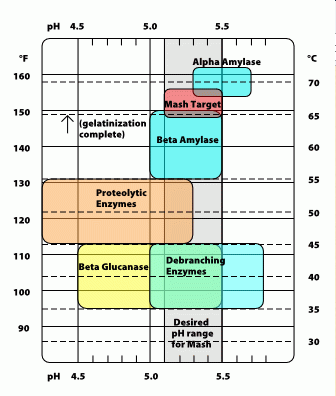
\includegraphics[width=0.75\linewidth]{./img/acaoenzimatica.png}
	\end{center}
	\legend{Fonte: adaptado de \citeonline{palmer2006}.}
\end{figure}

\begin{table}[]
\centering
\caption{Principais enzimas e suas temperatura de denaturação, faixa de trabalho e função.}
\label{Enzimas}
\begin{tabular}{ccccc}
\hline
\textbf{Enzimas} & \textbf{Faixa de Trab.} & \textbf{PH} & \textbf{Denaturação} & \textbf{Função}                                                                           \\ \hline
Beta Glucanase   & 35-45°C                 & 4.5-5.5     & 60°C                 & \begin{tabular}[c]{@{}c@{}}Atua na gelatinização; \\ Quebra o glucano.\end{tabular}       \\ \hline
Peptidase        & 45-55°C                 & 4.6-5.3     & 63°C                 & \begin{tabular}[c]{@{}c@{}}Libera amino nitrogênios.\\ Solubiliza proteínas\end{tabular}  \\ \hline
Protease         & 45-55°C                 & 4.6-5.3     & 68°C                 &  Diminui a turvação.                                                      \\ \hline
Beta Amylase     & 55-65°C                 & 5.0-5.5     & 71°C                 & Produz a maltose.                                                                         \\ \hline
Alpha Amylase    & 67-72°C                 & 5.3-5.7     & 77°C                 & \begin{tabular}[c]{@{}c@{}}Produz diversos açúcares,\\  incluindo a maltose.\end{tabular} \\ \hline
\end{tabular}
\end{table}



O lúpulo é uma flor que possui diversos óleos essenciais e resinas. Esta flor possui uma característica conservante que foi um dos motivos da sua inserção na cerveja.  Os alfa-ácidos são resinas que conferem o amargor da cerveja e que só são solúveis em água através do processo de isomerização que necessita de temperaturas elevadas para acontecer. Além dessas resinas, o lúpulo fornece à cerveja óleos essenciais que contribuem no aroma da bebida. Estes óleos são altamente voláteis, sendo eliminados caso o processo de fervura seja prolongado.

A levedura é um fungo que, através do processo de fermentação em ambiente anaeróbico, adquire energia quebrando os açúcares em gás carbônico e alcool etílico. Existem diversas espécies de levedura, a mais utilizada no processo de fermentação de cerveja é a \textit{Saccharomyces cerevisiae}. Por ser um ser vivo, é o ingrediente mais delicado, possuindo restrições maiores à temperatura de armazenamento e de inserção no mosto\footnote{Líquido açucarado destinado a fermentação}. Na fabricação de cerveja elas são classificadas em: levedura lager, de baixa fermentação em baixas temperaturas (6 a 15 °C), tem maior tempo de fermentação e menor formação de espuma no topo do fermentador. Leveduras de alta fermentação em temperaturas mais elevadas (14 a 25 °C), tem menor tempo de fermentação e maior formação de espuma no topo do fermentador.


%\begin{figure}[htb]
%	\caption{\label{fig_MUAP_comp}Soma de potenciais de ação das $n$ fibras de uma unidade motora, formando uma MUAP $h(t)$.}
%	\begin{center}
%	    \includegraphics[width=0.75\linewidth]{./img/MUAP_oneMU.png}
%	\end{center}
%	\legend{Fonte: adaptado de \citeonline{Basmajian1985}.}
%\end{figure}

%=========================================================================
		\section{Processo de Fabricação}
%-------------------------------------------------------------------------
O processo de fabricação de cerveja é longo e pode ter a duração variada de uma semana a alguns meses, dependendo do tempo de maturação e fermentação de cada cerveja. As etapas que demandam maior trabalho humano estão na produção do mosto, que deve compreender a mosturação, filtração, fervura e resfriamento. Este processo pode ter duração de 4 a 8 horas. 

Existem diversas formas de posicionamento dos caldeirões utilizados na brassagem, como por exemplo o \textit{Brewstand} (Figura \ref{brewstand}). Esta configuração utiliza 3 caldeirões em diferentes alturas, assim eliminando a necessidade de bombas para a transferência de líquidos entre recipientes. O primeiro caldeirão, mais elevado, é utilizado como reservatório de água quente para os processos de mosturação e lavagem. No segundo, a meia altura, é realizada a brassagem, filtração e lavagem. Este caldeirão deve ser equipado de fundo falso para impedir a passagem dos grãos. No terceiro é realizada a fervura e deve possuir serpentina para resfriamento ou ser acoplado um sistema refrigerador separado.   

\begin{figure}[htb]
	\caption{\label{brewstand} Estrutura em que é posicionada os caldeirões.}
	\begin{center}
	    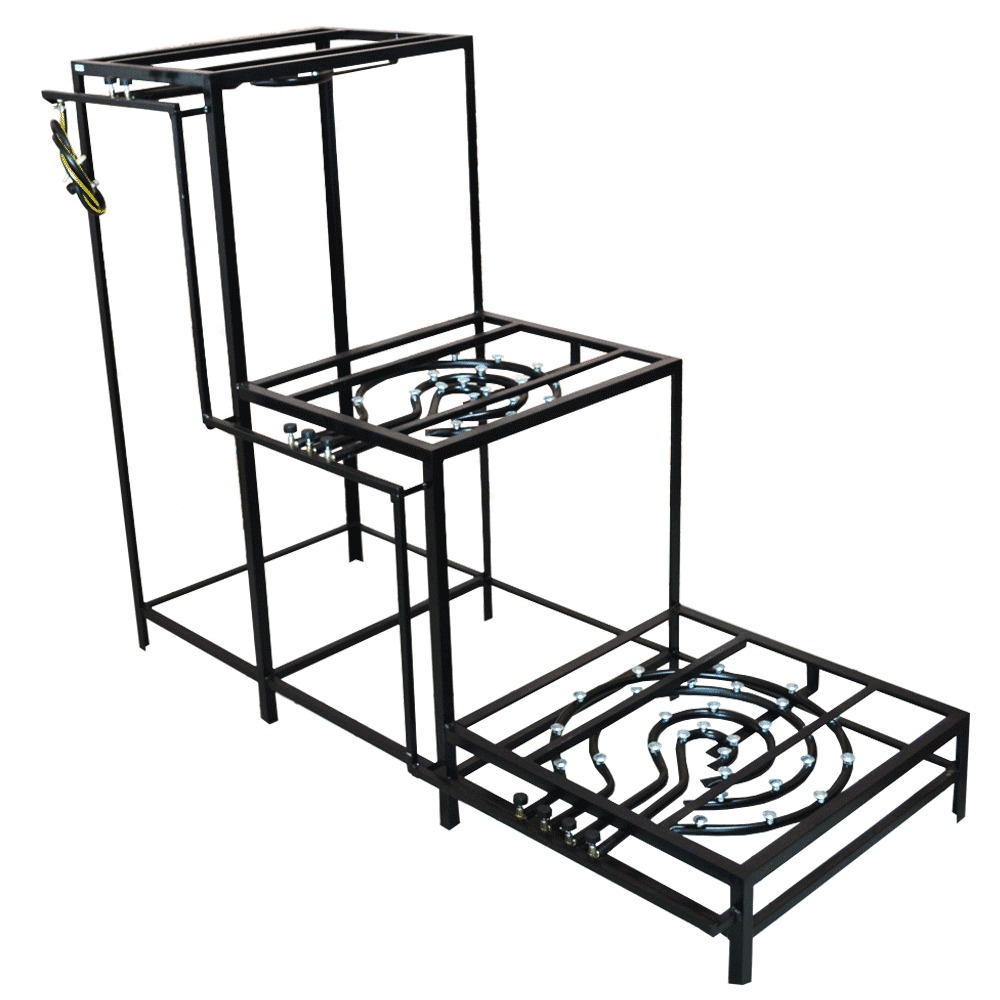
\includegraphics[width=0.75\linewidth]{./img/brewstand.jpg}
	\end{center}
	\legend{Fonte: Sitio de venda da Indupropil, fabricante da estrutura.}
\end{figure}



%-------------------------------------------------------------------------
				\subsection{Mosturação}
O processo de transformação das matérias-primas cervejeiras (água, malte, lúpulo e adjunto) em mosto, denomina-se mosturação ou brassagem \cite{venturini2001}. Nesta etapa, o malte moído é misturado com água quente no recipimente chamado mosturador. De forma que a mistura de água e malte deve se manter constante na temperatura da enzima que se deseja ativar. Cada patamar de temperatura é chamado de rampa de temperatura. Em uma brassagem podem existir de uma a quatro rampas de temperatura, dependendo do resultado em que se deseja o produto final. 

Em geral, no processo artesanal, a mosturação tem duração de 45 minutos a 2 horas, dependendo da técnica utilizada, quantidade de rampas e o tempo do aquecimento. É importante que a temperatura de todo o mosto esteja na faixa da enzima que se deseja ativar. Um dos métodos mais eficientes para a homogenização da temperatura é realizar constante agitação do mosto através de espátulas ligadas a um motor elétrico provido de redução, porém desta forma as espátulas necessitam ser de alumínio, inox ou plástico alimentício, assim como o restante do equipamento. O motor deve ser de potência suficiente para movimentar o líquido viscoso gerado pela mistura da água com os grãos e é necessário a construção de um suporte para fixação do motor e redução. Esta limitação de material torna o método caro para produção caseira. 

Um método alternativo é a utilização de uma bomba para recirculação do líquido no leito filtrante. Neste processo, o mosto é retirado pela base do caldeirão (onde está a fonte de calor) e devolvido ao topo. A bomba, em geral, possui pás e câmara de inox ou plástico alimentício e não necessita de grande potência. Este método dispensa o uso de suporte para fixação da bomba. 

%=========================================================================
	\subsection{Rampas de Temperatura}
%=========================================================================
Um termo que será muito utilizado é rampa de temperatura ou apenas rampa. Ele se refere a um patamar de temperatura estável durante certo tempo na mosturação. Tem como objetivo a ativação de uma enzina ou um grupo de enzimas específico para conferir uma característica à cerveja.

Por exemplo, uma brassagem com 3 rampas de 15min cada nas temperaturas de 45°C, 55°C e 65°C significa: elevar a temperatura até 45°C e mantê-la constante por 15min; elevar a temperatura até 55°C e mantê-la constante por 15min; finalmente, elevar a temperatura até 65°C e mantê-la constante por mais 15min. Em geral, o tempo é contado a partir do momento que a temperatura atinge o valor especificado com tolerância de até 2°C.

%-------------------------------------------------------------------------

%-------------------------------------------------------------------------
				\subsection{Filtração e Lavagem}
A filtração tem como objetivo fazer a sepação das partes sólidas e insolúveis no mosto do líquido. Os sólidos são constituídos de cascas e produtos insolúveis do grão, formando a camada conhecida como leito filtrante ou torta de filtro.  Em geral, esta etapa é dividida em duas partes: a) o líquido é separado dos sólidos, atravessando o leito filtrante e indo para um outro reservatório; b) no topo da torta é adicionada água na temperatura de 75 °C e é extraída na base do reservatório. Esta etapa tem como objetivo a recuperação do extrato de malte que ainda está retido na parte sólida e é chamada de lavagem. Na lavagem, a temperatura escolhida é de 75 °C, pois a viscosidade do mosto favorece a retirada do extrato, as enzimas estão, em sua maioria, inativas, o desenvolvimento bacteriano está bloqueado e não há riscos de extrair substâncias das cascas, principalmente os taninos. 

A separação é realizada através de um fundo falso na base do mosturador. Em geral o aquecimento se encontra abaixo do fundo falso, assim evitando a queima dos grãos. Na mesma altura do aquecimento ou abaixo está a saída do líquido como mostrado na Figura \ref{filtracao}.

\begin{figure}[htb]
	\caption{\label{filtracao} Corte ilustrativo do mosturador.}
	\begin{center}
	    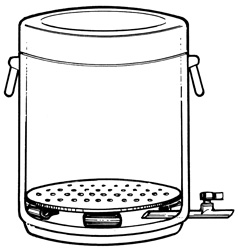
\includegraphics[width=0.55\linewidth]{./img/FalseBottom.jpg}
	\end{center}
	%\legend{Fonte: Adaptado de \citeonline{palmer2006}.}
\end{figure}

%-------------------------------------------------------------------------

%-------------------------------------------------------------------------
				\subsection{Fervura e Resfriamento}
Após a mosturação se inicia o processo de fervura do mosto, tendo como objetivos conferir estabilidade biológica do mosto, extrair o amargor das flores de lúpulo e coagular as proteínas presentes. No início desta etapa existe uma flora microbiana que resistiu as trocas de temperatura da mosturação e filtragem a qual é destruída na fervura ou reduzida a uma população incapaz de afetar a fermentação. Os alfa-ácidos do lúpulo, não solúveis em temperatura ambiente, são solubilizados na fervura através da isomerização, assim conferindo amargor a bebida. Com o aumento da temperatura, proteínas de maior cadeia carbônica, além de taninos, são coagulados formando o chamado \emph{trub}, que é um resíduo mucilaginoso semelhante a um lodo.

A fervura pode durar de 60 a 120 minutos e neste tempo ocorrem diversas adições de lúpulo em momentos distintos, dependendo da receita do cervejeiro. Em seguida o mosto é resfriado para uma temperatura em que seja possível a inoculação da levedura. O resfriamento também tem como objetivo a precipitação do \emph{trub} para a obtenção de uma cerveja mais límpida. Existem diversas formas de realizar o resfriamento como, por exemplo, serpentina imersa no mosto. 

%-------------------------------------------------------------------------

%-------------------------------------------------------------------------
				\subsection{Aeração, Fermentação e Maturação}
Ao final do processo de resfriamento o líquido está amargo e adocicado, em temperatura compatível a inoculação da levedura (16°C para leveduras ales e a 12°C em leveduras lager). Neste momento, o líquido é transferido para o fermentador, onde deve ser adicionado oxigênio, pois a levedura utiliza este composto no seu processo de multiplicação, ocasionando uma fermentação mais saudável. A adição pode ser realizada com agitação constante do mosto por alguns minutos, utilizando uma bomba de ar ligada a uma pedra difusora ou com cilindro de oxigênio hospitalar, sendo o último método o mais eficiente e também aquele com maior custo. Em geral, cervejeiros caseiros utilizam os dois primeiros métodos por questões de custo.

Com o mosto oxigenado, a levedura é adicionada e o fermentador é fechado, permanecendo apenas uma válvula de alívio para saída do gás carbônico. A fermentação deve ser realizada com temperatura controlada com o objetivo de aumentar a repetibilidade da receita. Em processos caseiros são usadas geladeiras e \emph{freezers} para o resfriamento e, no caso de atuação para elevação de temperatura, pode ser utilizada uma lâmpada incandescente ou resistências elétricas a seco. 

A fermentação acaba quando a levedura deixa de realizar a reação de quebra dos açúcares em álcool e gás carbônico. Isto pode ser ocasionado pelo consumo de todos os fermentáveis ou pelo alcance do limite de álcool da levedura. Ao fim da fermentação tem início o processo de maturação, onde, normalmente, a temperatura é reduzida a cerca de 0°C por 1 a 4 semanas. Este processo tem como principais objetivos a melhora do sabor da cerveja pela reabsorção de compostos realizada pela levedura e o auxílio a clarificação do líquido, pois a floculação do fermento é elevada ao se diminuir a temperatura.



%-------------------------------------------------------------------------
		\section{Conceitos de Automação}
%-------------------------------------------------------------------------
\label{sec:MTDs}

Entende-se por automação os sistemas computadorizados que substituem tarefas de trabalho humano de forma econômica e rápida \cite{Aguirre2007}. Portanto, automação é um conceito muito abrangente e que utiliza conteúdos de diferentes áreas da engenharia para um mesmo sistema. Porém existem conceitos e definições largamente utilizadas neste contexto a serem detalhadas nesta seção.


%-------------------------------------------------------------------------
			\subsection{Definição de Sistema}
%-------------------------------------------------------------------------
O termo sistema está relacionado a um conceito primitivo, cujo o entendimento é mais intuitivo do que propriamente assiociado a uma definição exata. O seu uso é difundido em praticamente todas as áreas do conhecimento humano, onde se encontram diferentes definições\cite{Aguirre2007}.

Esse conceito é amplamente utilizado em automação e é importante defini-lo neste contexto. Um sistema automático pode fazer parte de um sistema maior, assim como ser decomposto em diversos subsistemas e esses decompostos em outros e assim sucetivamente até serem alcançados componentes considerados elementares. Em geral, os sistemas podem ter seu comportamento descrito de forma simplificada através de modelos. \citeonline{Aguirre2007} define sistemas de automação como um conjunto de componentes interconectados que tomam ações através de lógicas predeterminadas, estado atual do equipamento e a ocorrência de eventos.
%-------------------------------------------------------------------------
				\subsection{Sistemas de Supervisão}
%-------------------------------------------------------------------------
Um sistema de supervisão tem como objetivo monitorar variáveis do sistema e possibilitar ao operador acesso ao monitoramento e controle de um determinado processo. A supervisão não é, necessariamente, instalada próxima aos sistemas que são supervisionados, podendo fornecer supervisionamento de um ou mais subsistemas. Em ambiente industrial, esses sistemas também são chamados de sistemas SCADA (\emph{Supervisory Control and Data Acquisition}), conforme exemplificados em diagrama na Figura \ref{filtracao01}.
Os sistemas de supervisão são ferramentas que atuam, controlam e comunicam com subsistemas utilizando interfaces homem-maquina (IHM) amigáveis para mostrar variáveis dos subsistemas supervisionados. Permitem, assim a centralização da informação de sistemas muitas vezes dispersos geograficamente ou presentes em ambientes complexos \cite{Rosario2005}. 

\begin{figure}[htb]
	\caption{\label{filtracao01} Diagrama de blocos de um sistema de supervisão.}
	\begin{center}
	    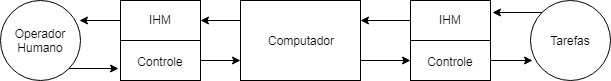
\includegraphics[width=0.75\linewidth]{./img/SistemaSCADA.jpg}
	\end{center}
	\legend{Fonte: Adaptado de \citeonline{Rosario2005}.}
\end{figure}


%-------------------------------------------------------------------------
			\subsection{Representação de Sistemas de Automação}
%-------------------------------------------------------------------------
Não existe uma padronização na representação dos projetos de sistemas de automação, porém existe a necessidade de utilizar uma descrição simplificada para sua correta compreensão. \citeonline{Aguirre2007} destaca três perpectivas principais, que com seus modelos, são capazes de fornecer uma descrição completa do sistema: perspectiva funcional, estrutural e comportamental.

A perspectiva funcional, como o nome evidência, tem como objetivo descrever a função do sistema, sendo por diagramas de circuito, Redes de Petri Canal/Agência, diagrama de fluxo de dados ou diagramas de blocos. A perspectiva estrutural tem como objetivo designar a organização, arranjo e construção do sistema, sendo realizada por desenhos mecânicos, diagramas Entidade/Relacionamento, mapas ou orientação por objetos. A perspectiva comportamental fornece uma noção temporal ou sequencial ao sistema, descrevendo quando cada ação irá ocorrer, podendo ser por autômatos, redes de Petri marcadas ou ainda por equações booleanas. 

%-------------------------------------------------------------------------
			\subsection{Processos Térmicos}
%-------------------------------------------------------------------------
Conforme descrito na seção 2.2, a produção de cerveja é composta por uma série de processos térmicos, onde o objetivo principal é o aquecimento ou resfriamento de líquidos. Do ponto de vista de controle, diversas técnicas pressupõem a existência de um modelo que descreve o sistema de interesse. Conforme a modelagem de \citeonline{Controle2005}, sistemas térmicos podem ser representados de forma simplificada por uma resistência elétrica que injeta energia térmica em um ambiente, sendo a variável manipulada a tensão elétrica e a variável de processo a temperatura. Usando essa modelagem como base foi realizado o equacionamento para um sistema, mas considerando a queima de gás de cozinha como injetor de energia térmica no ambiente e a variável manipulada sendo a vazão.

Considerando uma mudança infinitesimal na energia do sistema ocasione uma mudança infinitesimal na temperatura
 \begin{equation}
	\label{eq:1}
	dQ = C \times dT,
\end{equation}
onde C é a capacidade térmica do material. Então a sua variação ao longo do tempo pode ser representada por

\begin{equation}
	\label{eq:2}
	\frac{dQ}{dt} =C \times \frac{dT}{dt}.
\end{equation}
A troca de energia térmica é dada pela potência fornecida pela queima do gás e pela perda de energia para o ambiente, sendo esta última dependente da diferença de temperatura entre o material e o ambiente. Tal que

\begin{equation}
	\label{eq:3}
	\frac{dQ}{dt} =P-k_T \times (T-T_a).
\end{equation}

Sendo na equação (\ref{eq:3}), $P$ é a potência fornecida pela combustão, $k_T$ é a constante de perdas, T é a temperatura do material e $T_a$ é a temperatura ambiente. Combinando as equações (\ref{eq:3}) e (\ref{eq:1}) obtém-se


\begin{equation}
	\label{eq:4}
	C \times\frac{dT}{dt}+k_T\times T=P+k_T\times T_a.
\end{equation}

A partir da aplicação da Transformada de Laplace em  (\ref{eq:4}) se tem que a dinâmica que descreve a temperatura é dada por

\begin{equation}
	\label{eq:5}
	T(s)=\frac{1}{Cs+k_T}\times P(s) + \frac{k_T}{Cs+k_T}T_a(s).
\end{equation}
Porém este modelo considera que a temperatura no sistema é homogênea, ou seja, a potência injetada pela queima é instantaneamente distribuída e detectada pelo instrumento de medição, o que é apenas alcançado em regime permanente. Entretanto este fenômeno de heterogeneidade pode ser aproximado pela introdução de um atraso na função de transferência que relaciona a potência com a temperatura, chegando no modelo final:

\begin{equation}
	\label{eq:6}
	\frac{T(s)}{P(s)}=\frac{e^{-\tau s}}{Cs+k_T}.
\end{equation}
%=========================================================================
	\chapter{Solução de Hardware}
Este capítulo explica a estrutura física, sensoriamento, atuação e placas eletrônicas utilizados na execução do projeto.


%=========================================================================
		\section{Posicionamento dos caldeirões e estrutura mecânica}
%-----------------------------------------------------------------------------------------------------------------------------------
Foi escolhido o posicionamento dos caldeirões em forma de cascata, como ilustrado no \textit{Brewstand} da Figura \ref{brewstand}, onde o nível inferior do primeiro caldeirão deve estar acima do nível superior do segundo, sendo a mesma configuração observada no nível do segundo e o terceiro caldeirões. Dessa forma a passagem de líquidos entre os caldeirões poderia ser realizada sem o auxílio de bombas. No caldeirão superior está a água que será utilizada para a lavagem, no intermediário seria realizada a mostura e no inferior ocorrerá a fervura e resfriamento. Na figura \ref{brewstand} está a estrutura utilizada sem os componentes da automação. Com esta configuração, o controle de passagem de líquido seria realizado com válvulas solenóides de material metálico que são componentes de menor custo em relação a bombas. Porém ao realizar os testes com as válvulas solenóides notou-se que estas não permitem uma vazão de transferência adequada devido à baixa pressão decorrente da coluna de água. Portanto escolheu-se mudar o fluxo do processo e utilizar bombas para transferência de líquido. Nesta nova configuração, o caldeirão inferior passa a ser o recipiente da água da lavagem, o intermediário continua sendo o de mosturação e o superior passa a ser o de fervura.

A estrutura apresentada na Figura \ref{brewstand} é constituída de cantoneiras de aço de uma polegada com pintura preta, possui 147 centímetros de altura, 78,3 centímetros de largura e 162 centímetros de comprimento. Segundo \citeonline{Indupropil}, esta estrutura foi projetada para suportar uma brassagem de 100 litros. O módulo superior possui 10 queimadores e duas válvulas reguladoras de gás, o intermediário possui 20 queimadores e 3 reguladoras e o inferior possuí 30 queimadores e 4 válvulas. A transmissão de gás entre queimadores é realizada por tubulação de mesmo material afixada na estrutura e a entrada de gás é conectada através de uma mangueira flexível. Como a estrutura utilizada foi projetada para um volume de produção muito superior ao desejado, não é necessário controlar todas as válvulas reguladoras existentes,  sendo controlada apenas uma em cada módulo.

A planta inteira do sistema é apresentada na Figura \ref{plantaPronta}. Circuladas em vermelho estão as bombas de passagem. Apontada em vermelho, atrás do caldeirão 1, está a bomba de recirculação. Percebe-se que existe uma tubulação de gás ao lado esquerdo da estrutura e sobre os registros de gás estão os servomotores circulados em verde. As placas eletrônicas, microcontrolador e \textit{notebook} estão ao lado do \textit{brewstand} circulados em azul. 
\begin{figure}[htb]
	\caption{\label{plantaPronta}Foto da planta com seus atuadores e controle.}
	\begin{center}
	    \includegraphics[width=0.85\linewidth]{./img/sistemaInteiro02.jpg}
	\end{center}
	%\legend{Fonte: Adaptado de \citeonline{Rosario2005}.}
\end{figure}

%=========================================================================
		\section{Componentes de automação e controle}
%-----------------------------------------------------------------------------------------------------------------------------------
Para alimentar os atuadores de tensão contínua foi utilizada uma fonte de tensão ATX conforme ilustrada na Figura \ref{FonteAlimentacao}. Com capacidade de corrente de 12A na tensão de 5V, sua aplicação usual é para alimentação de computadores e apresentam baixo custo.

\begin{figure}[htb]
	\caption{\label{FonteAlimentacao}Fonte de tensão ATX.}
	\begin{center}
	    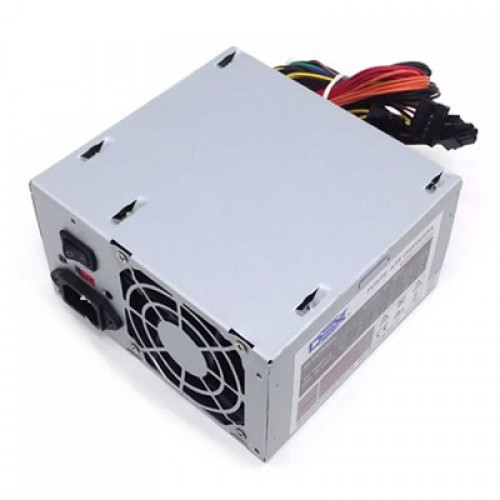
\includegraphics[width=0.45\linewidth]{./img/fonteATX.jpg}
	\end{center}
	%\legend{Fonte: Adaptado de \citeonline{Rosario2005}.}
\end{figure}

%=========================================================================
		\section{Arduino Uno}
%-----------------------------------------------------------------------------------------------------------------------------------
Com o objetivo de fazer a leitura dos sensores, envio de dados via comunicação serial ao Notebook e receber os comandos de atuação
do supervisório, foi utilizada um placa de desenvolvimento Arduino Uno e sua IDE para a compilação. Na Figura 7 é apresentada a placa utilizada e na Figura 8 ilustrado o fluxo de dados do sistema.

\begin{figure}[htb]
	\caption{\label{ArduinoUno}Placa Arduino Uno.}
	\begin{center}
	    \includegraphics[width=0.45\linewidth]{./img/ArduinoUno.jpg}
	\end{center}
	%\legend{Fonte: Adaptado de \citeonline{Rosario2005}.}
\end{figure}


  \begin{figure}[htb]
	\caption{\label{diagramaHardware}Esquemático do fluxo de dados do sistema.}
	\begin{center}
	    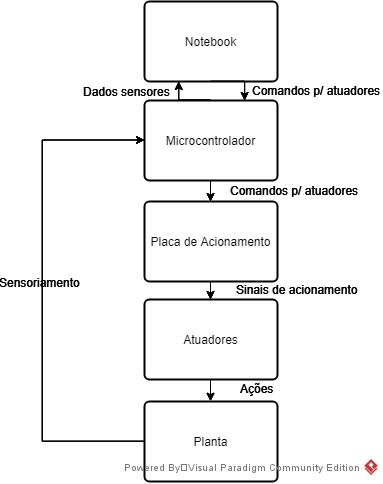
\includegraphics[width=0.55\linewidth]{./img/Eletronicadiagrama.jpg}
	\end{center}
	%\legend{Fonte: Universidade Tecnológica Federal do Paraná - Coordenação de Engenharia Eletrônica -  Aula 7 - Prof. Leandro Castilho Brolin.}
\end{figure}

A placa utilizada é composta por um microcontrolador ATMEGA328p, possuindo 14 pinos digitais e 6 analógicos. Como não houve necessidade de utilizar os conversores A/D do microcontrolador, os pinos analógicos foram utilizados como digitais. Na Tabela \ref{Pinagem} está a relação dos pinos utilizados e sua função. Todos os pinos digitais do microcontrolador são utilizados e seus pinos analógicos são utilizados como digitais para leitura de sinais booleanos dos sensores.

\begin{table}[]
\caption{Relação dos pinos utilizados.}
\label{Pinagem}
\begin{tabular}{cccc}
\hline
\textbf{Pino Digital} & \textbf{Função}          & \textbf{Pino Analógico} & \textbf{Função}   \\ \hline
0                     & Rx - Comunicação Serial    & A0                      & Sensor de Chama 1 \\ \hline
1                     & Tx - Comunicação Serial  	 & A1                      & Sensor de Chama 2 \\ \hline
2                     & Sensor de Temperatura 1  & A2                      & Sensor de Chama 3 \\ \hline
3                     & Buzzer                  		 & A3                      & Sensor de Nível 1 \\ \hline
4                     & Bomba de Resfriamento     & A4                      & Sensor de Nível 2 \\ \hline
5                     & Bomba de Recirculação      & A5                      & Sensor de Nível 3 \\ \hline
6                     & Bomba de Transferência 3 &                         &                   \\ \hline
7                     & Bomba de Transferência 2 &                         &                   \\ \hline
8                     & Válvula Solenóide 1           &                         &                   \\ \hline
9                     & Servomotor 3             	&                         &                   \\ \hline
10                    & Servomotor 2             	&                         &                   \\ \hline
11                    & Servomotor 1             	&                         &                   \\ \hline
12                    & Sensor de Temperatura 2  &                         &                   \\ \hline
13                    & Sensor de Temperatura 3  &                         &                   \\ \hline
\end{tabular}
\end{table}

%=========================================================================
		\section{Placa de Acionamentos}
%-----------------------------------------------------------------------------------------------------------------------------------

Para automação do sistema foram utilizados os atuadores da Tabela \ref{Atuadores}. Percebe-se que são utilizados 5 atuadores que trabalham em tensão alternada de 220 $Vrms$ e 4 atuadores que utilizam a tensão contínua de 5 $V$. Com o objetivo principal de isolar eletricamente os atuadores de tensão alternada, foi construída uma placa de circuito impresso para acioná-los, conforme desenho 3D apresentado na Figura \ref{PlacaAcionamento}. Os sinais de ativação provém do microcontrolador, passam pelo optoacoplador \textit{4N25} e polarizam um transistor que aciona o relé. No caso dos servomotores e do \textit{Buzzer} não há necessidade de transistores e relés.




\begin{table}[]
\caption{Atuadores utilizados.}
\label{Atuadores}
\begin{tabular}{cccc}
\hline
\textbf{Atuador}      & \textbf{Quantidade} & \textbf{Acionamento} & \textbf{Objetivo}            \\ \hline
Bomba não submersível & 3                   & 220 Vrms             & Recirculação e transferência \\ \hline
Bomba Submersível     & 1                   & 220 Vrms             & Resfriamento do mosto        \\ \hline
Válvula Solenóide     & 1                   & 220 Vrms             & Entrada de água              \\ \hline
Servomotor            & 3                   & PWM - 5Vdc           & Controle de fluxo de gás     \\ \hline
Buzzer                & 1                   & 5 Vdc                & Avisos sonoros               \\ \hline
\end{tabular}
\end{table}




\begin{figure}[htb]
	\caption{\label{esquematicoAcionamentos}Esquemático do acionamento dos relés.}
	\begin{center}
	    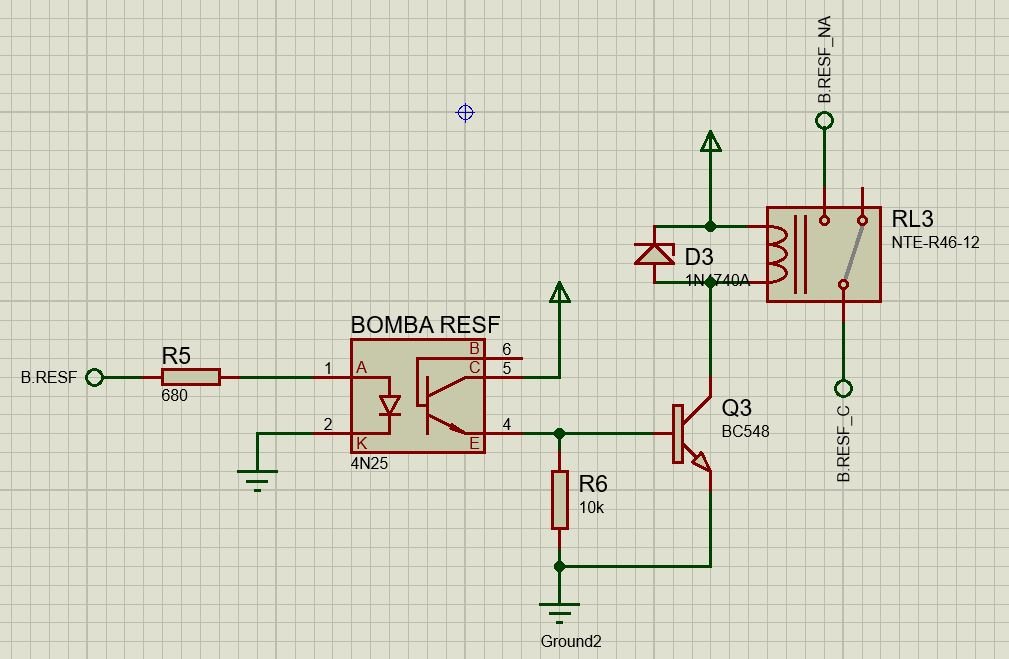
\includegraphics[width=0.75\linewidth]{./img/esquematicoAcionamento01.jpg}
	\end{center}
	%\legend{Fonte: Universidade Tecnológica Federal do Paraná - Coordenação de Engenharia Eletrônica -  Aula 7 - Prof. Leandro Castilho Brolin.}
\end{figure}

Analisando o circuito da Figura \ref{esquematicoAcionamentos} segue que o resistor R5 é de 680 ohms, valor escolhido para que a corrente sobre o diodo do optoacoplador seja de aproximadamente 5 mA. Esta corrente é suficiente para polarizar do transistor sem sobrecarregar o consumo do microcontrolador. O diodo D3 é um diodo zener de 16V de tensão reversa colocado para evitar picos de tensão causados pelo chaveamento da bobina do relé. O resistor R6 é conectado na base do transistor e ao terra com o objetivo de evitar o acionamento do relé caso não haja sinal na porta do Arduino. Os atuadores são ligados na porta normalmente aberta garantindo que não sejam ligados caso não exista sinal. 

  \begin{figure}[htb]
	\caption{\label{esquematicoAcionamentos2}Esquemático do acionamento dos servomotores.}
	\begin{center}
	    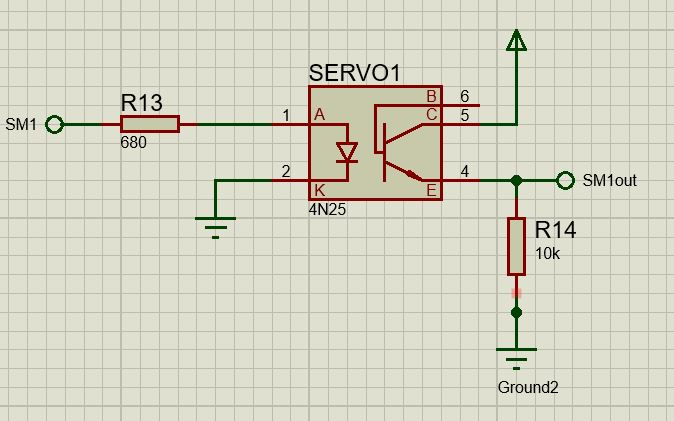
\includegraphics[width=0.75\linewidth]{./img/esquematicoAcionamento02.jpg}
	\end{center}
	%\legend{Fonte: Universidade Tecnológica Federal do Paraná - Coordenação de Engenharia Eletrônica -  Aula 7 - Prof. Leandro Castilho Brolin.}
\end{figure}

O isolamento dos servomotores é mostrado na figura \ref{esquematicoAcionamentos2}. Ele é realizado da mesma forma que as bombas, mas sem a utilização dos transistores e relés. Utilizando esses circuitos foi desenhada a placa de circuito impresso e construída utilizando o processo de fotolitografia e corrosão via percloreto de ferro. A placa pronta está na figura \ref{placaPronta}.

  \begin{figure}[htb]
	\caption{\label{placaPronta}Placa de circuito impresso construída.}
	\begin{center}
	    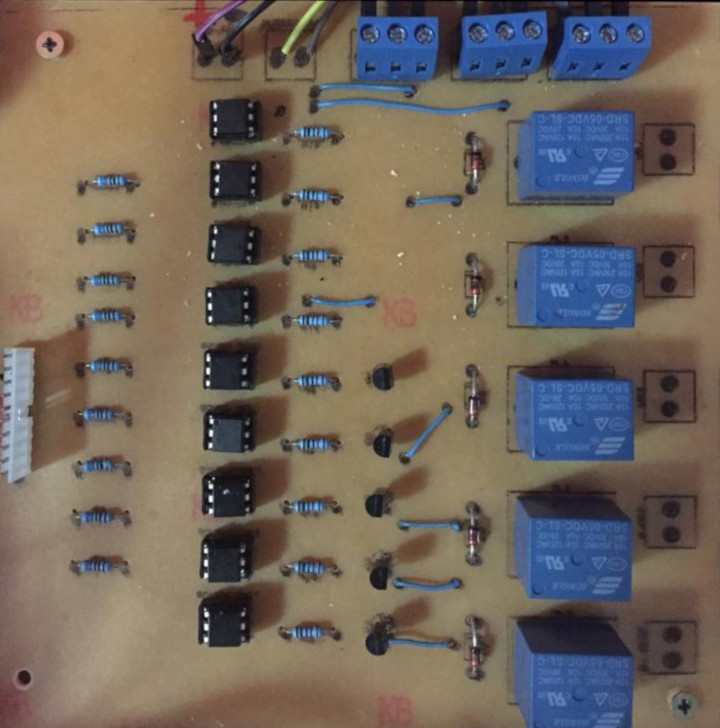
\includegraphics[width=0.55\linewidth]{./img/placaPronta.jpg}
	\end{center}
	%\legend{Fonte: Universidade Tecnológica Federal do Paraná - Coordenação de Engenharia Eletrônica -  Aula 7 - Prof. Leandro Castilho Brolin.}
\end{figure}

\begin{figure}[htb]
	\caption{\label{PlacaAcionamento}Modelo 3D da Placa de Acionamento Construída.}
	\begin{center}
	    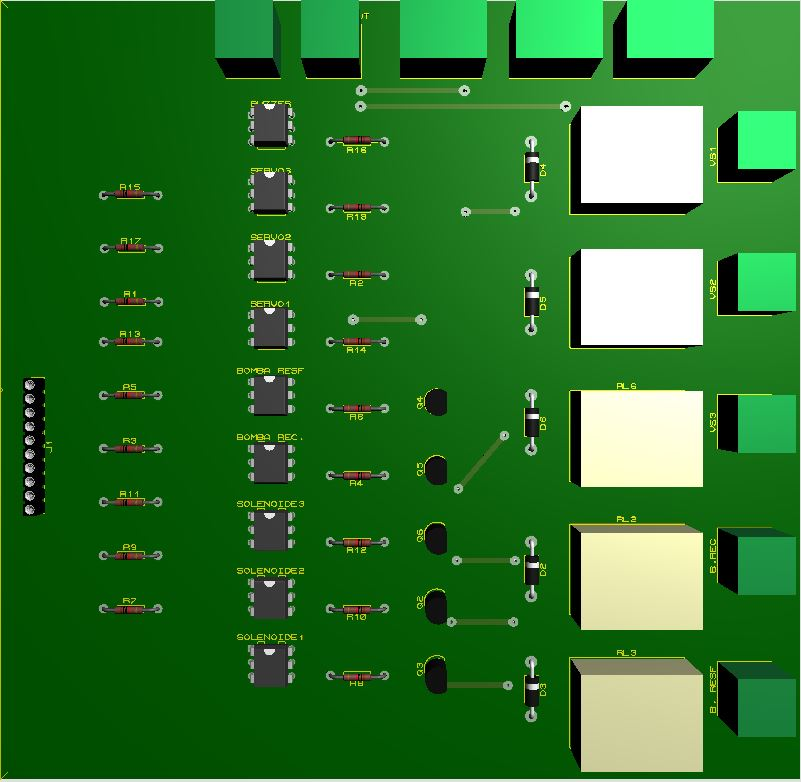
\includegraphics[width=0.45\linewidth]{./img/PlacadeAcionamentos.jpg}
	\end{center}
	%\legend{Fonte: Adaptado de \citeonline{Rosario2005}.}
\end{figure}


%=========================================================================
		\section{Sensor de Nível}
%-----------------------------------------------------------------------------------------------------------------------------------
Foi escolhido um sensor tipo bóia construído completamente em inox. Quando o nível do líquido está abaixo da bóia, o sensor está com os contatos fechados, caso contrário está com os contatos abertos. Suas principais características são a operação em temperaturas de até 120°C, 0,5 Ampéres de corrente elétrica e  0,1 Ohms de resistência elétrica.   
\begin{figure}[htb]
	\caption{\label{SensordeNivel}Sensor de nível utilizado.}
	\begin{center}
	    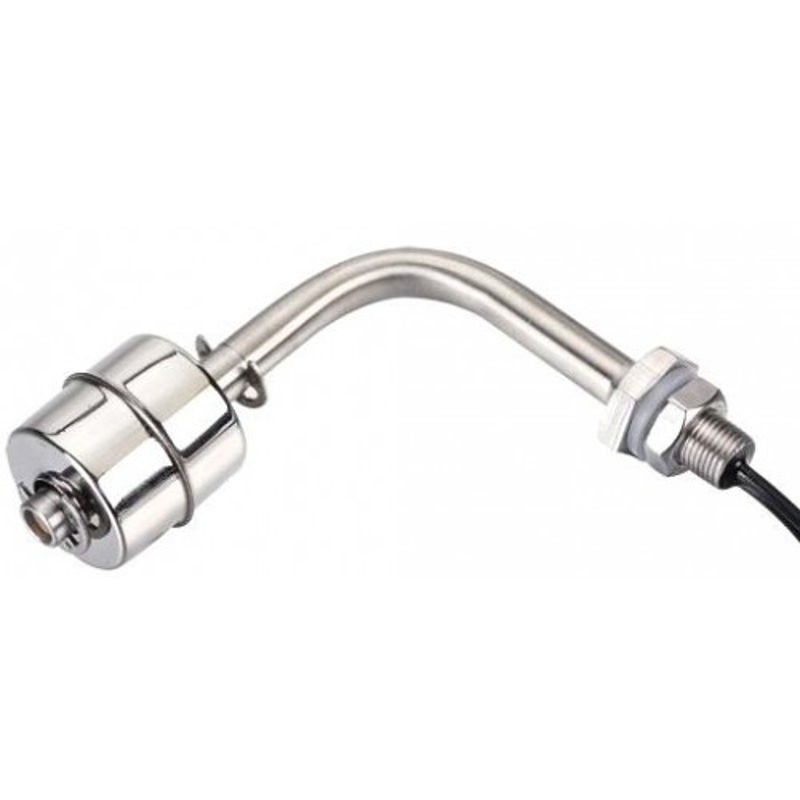
\includegraphics[width=0.45\linewidth]{./img/SensordeNivel.jpg}
	\end{center}
	%\legend{Fonte: Adaptado de \citeonline{Rosario2005}.}
\end{figure}

%=========================================================================
		\section{Sensor de Temperatura}
%-----------------------------------------------------------------------------------------------------------------------------------
Foi escolhido o sensor DS18B20 por apresentar saída digital por um único fio, dispensa portanto o uso de conversores A/D. Na faixa de -10°C a 85°C, este sensor possui máximo erro de 0,5°C e na faixa de -30°C a 100°C possui erro máximo de 1°C , os quais são aceitáveis tendo em vista o processo considerado.

\begin{figure}[htb]
	\caption{\label{SensordeTemperatura}Sensor de Temperatura DS18B20 com encapsulamento em inox.}
	\begin{center}
	    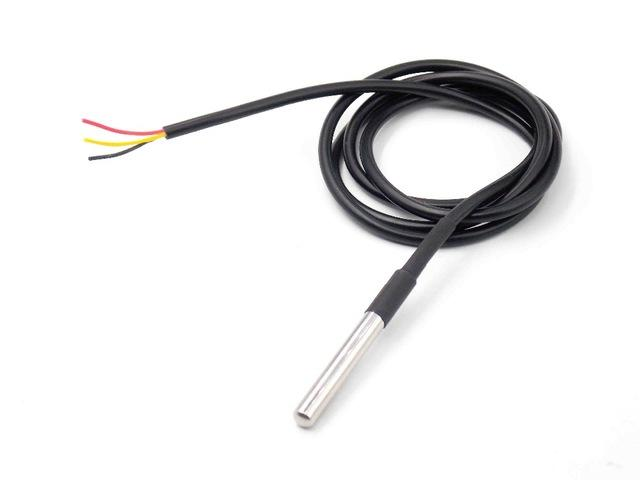
\includegraphics[width=0.45\linewidth]{./img/SensordeTemperatura.jpg}
	\end{center}
	%\legend{Fonte: Adaptado de \citeonline{Rosario2005}.}
\end{figure}

%=========================================================================
		\section{Sensor de Chama}
%-----------------------------------------------------------------------------------------------------------------------------------
Os sensores de chama não foram instalados, pois requerem modificação na estrutura e necessitam elevado tempo de calibração. Por esta razão foi colocada uma chama piloto em cada queimador evitando o vazamento de gás. Tanto os sensores de nível quanto os de chama geram sinais booleanos e são conectados em pinos analógicos programados para funcionarem como digitais. Embora não instalados, a lógica de recebimento do sinal foi programada, facilitando uma futura utilização.


%=========================================================================
		\section{Bombas}
%-----------------------------------------------------------------------------------------------------------------------------------
São utilizadas bombas para as transferências entre caldeirões, para recirculação do mosto e para bombear água na serpentina de resfriamento. Nas duas primeiras funções são utilizadas bombas de pás retas com 34 W de potência e que, segundo o fornecedor, possui 1 metro de coluna de água e vazão de 60 litros por hora. Sua principal utilização é em máquinas de lavar roupa, mas sendo adaptadas com a câmara e pás em inox para a utilização no processo de fabricação de cerveja. Essa bomba é mostrada na Figura \ref{Bomba01}.
\begin{figure}[htb]
	\caption{\label{Bomba01}Bomba de pás retas utilizada.}
	\begin{center}
	    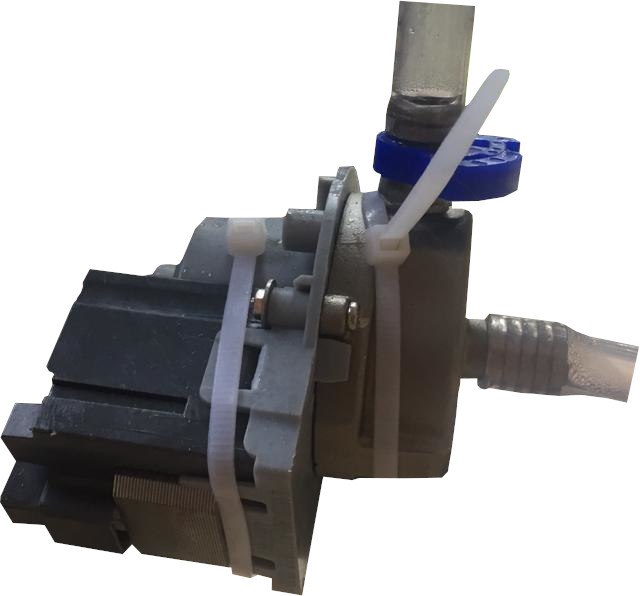
\includegraphics[width=0.45\linewidth]{./img/Bomba01.jpg}
	\end{center}
	%\legend{Fonte: Adaptado de \citeonline{Rosario2005}.}
\end{figure}

%=========================================================================
		\section{Válvula Solenóide}
%-----------------------------------------------------------------------------------------------------------------------------------
Para o processo é utilizada água encanada com controle de entrada realizado através da válvula solenóide da Figura \ref{Solenoide}. Ao aplicar 220 Volts nos terminais da válvula ela permite a passagem do líquido. Porém essa passagem não é controlada proporcionalmente, portanto não há controle da variável de vazão, apenas se há entrada ou não entrada de água. 
\begin{figure}[htb]
	\caption{\label{Solenoide}Válvula Solenóide.}
	\begin{center}
	    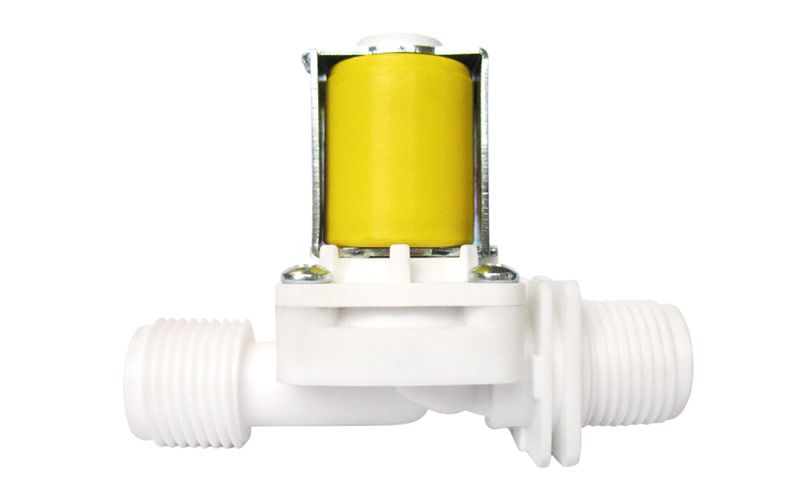
\includegraphics[width=0.45\linewidth]{./img/Solenoide.jpg}
	\end{center}
	%\legend{Fonte: Adaptado de \citeonline{Rosario2005}.}
\end{figure}
%=========================================================================
		\section{Servomotor}
%-----------------------------------------------------------------------------------------------------------------------------------
Em aplicações de controle, a saída de gás é usualmente controlada via válvulas solenóides proporcionais, as quais possuem preço elevado. Uma forma de substituição é utilizar um servomotor para controlar a abertura do registro de gás. O servomotor escolhido foi o \textit{MG995}, que possui torque de aproximadamente 10 $kgf.cm$ na tensão de 5 $V$. Ele é controlado através do \textit{Duty-Cycle} de um sinal PWM (\textit{Pulse Width Modulation}) de 500 Hz. O servomotor pode varias seus graus de 0 a 180 conforme o sinal PWM em sua entrada, sendo 50\% de \textit{Duty-Cycle} para 0° e 100\%  para 180°. Na Figura \ref{ServoMotor} é apresentado o modelo utilizado. 
\begin{figure}[htb]
	\caption{\label{ServoMotor}Servomotor modelo \textit{MG995}.}
	\begin{center}
	    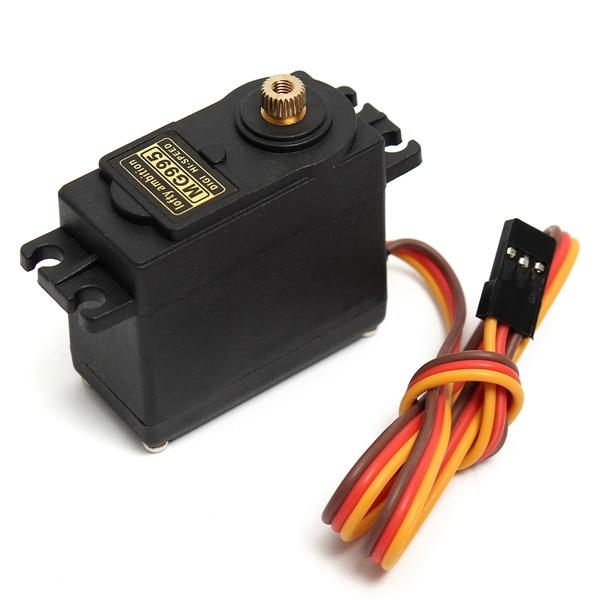
\includegraphics[width=0.45\linewidth]{./img/ServoMotor.jpg}
	\end{center}
	%\legend{Fonte: Adaptado de \citeonline{Rosario2005}.}
\end{figure}

%=========================================================================
% Controle de Temperatura
	\chapter{Controle de Temperatura}
Neste capítulo será descrita a técnica utilizada para a identificação dos parâmetros da planta e projeto de um controlador PI visando o controle da temperatura dos caldeirões.

%=========================================================================
		\section{Modelagem Experimental da Planta}
%-----------------------------------------------------------------------------------------------------------------------------------
Na revisão bibliográfica foi visto que um processo térmico pode ser modelado como um sistema de primeira ordem com um atraso. A partir de ensaios na planta, verificou-se que o atraso da planta em questão é muito menor que o seu tempo de acomodação, não será considerado na modelagem. Assim, o objetivo é identificar um modelo na forma
\begin{equation}
	\label{eq:7}
	G(s)=\frac{K}{Ts+1},
\end{equation}
onde $T$ é constante de tempo e $K$ o ganho estático do processo. Ao se aplicar um salto no sistema e registrar o tempo para este se acomodar é possível obter o valor da constante de tempo. Portanto foi aberto o registro de gás em 15 graus e foram registrados os dados de temperatura do caldeirão ao longo do tempo, conforme apresentado na Figura \ref{Salto02}. Este experimento foi realizado utilizando o módulo intermediário do \textit{brewstand} com o caldeirão de 45 litros, recirculação ligada e 30 litros de água. Essas configurações foram escolhidas para se aproximar ao máximo do processo de mosturação da planta. A acomodação do sistema aconteceu na temperatura de 92°C em cerca de 1 hora e 15 minutos. Para atingir 63\% da temperatura de acomodação levou-se o tempo de 1900 segundos, valor o qual corresponde a constante de tempo do sistema.
 
\begin{comment}
\begin{figure}[htb]
	\caption{\label{Salto01}Resposta ao salto da planta com abertura de 5°.}
	\begin{center}
	    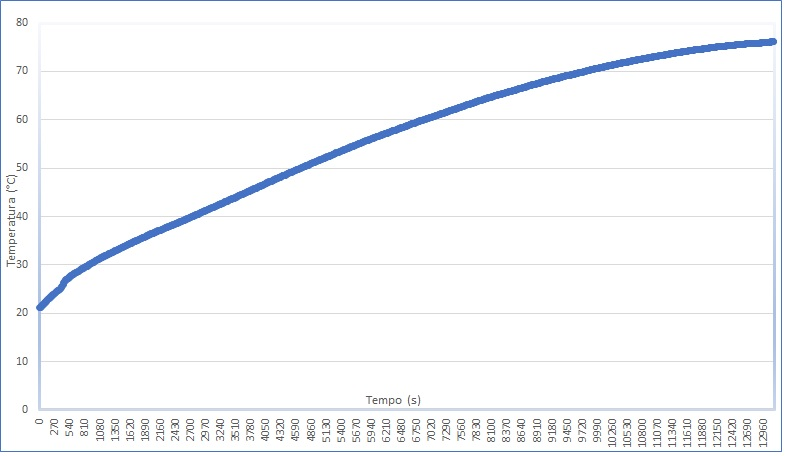
\includegraphics[width=0.9\linewidth]{./img/Salto01.jpg}
	\end{center}
	%\legend{Fonte: Adaptado de \citeonline{Rosario2005}.}
\end{figure}
\end{comment}

O ganho estático representa o quanto o valor da entrada será escalonado na saída em regime permanente. A partir dos dados da Figura \ref{Salto02}, é possível determinar

\begin{equation}
	\label{eq:8}
	K=\frac{T_{max} - T_{min}}{^{\circ} max  - ^{\circ}min}  = \frac{92-35}{15-0} = 3.8   \frac{^{\circ}C}{^{\circ}}.
\end{equation}

\begin{figure}[htb]
	\caption{\label{Salto02}Resposta ao salto da planta com abertura de 15°.}
	\begin{center}
	    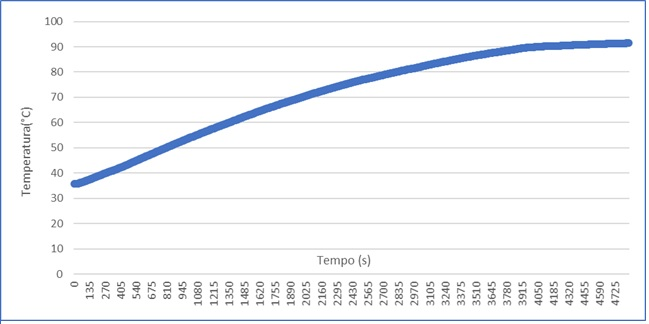
\includegraphics[width=0.9\linewidth]{./img/Salto02.jpg}
	\end{center}
	%\legend{Fonte: Adaptado de \citeonline{Rosario2005}.}
\end{figure}

Assim, para fins de projeto, será considerado que a variação da temperatura a partir da abertura da válvula de gás é representada pela seguinte função de transferência:

\begin{equation}
	\label{eq:9}
	G(s)=\frac{3.8}{1900s+1} = \frac{0.002}{s+0.000526} 
\end{equation}

%-----------------------------------------------------------------------------------------------------------------------------------
		\section{Definição do Controlador}
%-----------------------------------------------------------------------------------------------------------------------------------
Com a planta modelada, é possível utilizar a técnica de Lugar das Raízes para achar o controlador ideal para esta planta. Primeiro se deve definir o tipo de controlador que se deseja. Tendo em vista a aplicação, foi escolhido um controle proporcional integrativo, pois o mesmo garante erro nulo em regime permanente para sinais do tipo salto ou degrau. Deve-se levar em conta também que não é aceitável \textit{overshoot}, pois se o mosto atingir temperaturas maiores que 75 graus as enzimas do malte denaturam.

Utilizou-se a ferramenta \textit{rltool} do programa \textit{MATLAB} para encontrar o controlador desejado. O zero do controlador foi posicionado próximo ao polo da planta, assim diminuindo significantemente o tempo de acomodação. Esta escolha implica em uma resposta mais lenta aos distúrbios de entrada, mas como o processo não prevê nenhum distúrbio dessa natureza durante a mosturação, esta característica não afeta o desempenho geral do sistema em malha fechada. Na Figura \ref{RootLocus} é apresentado o LGR dos dos polos do sistema em malha fechada para o controlador (\ref{eq:10})
 
\begin{equation}
	\label{eq:10}
	C(s)=K(\frac{s+\frac{1}{T_i}}{s}) = 5.25(\frac{s+0.00035}{s})  
\end{equation}

\begin{figure}[htb]
	\caption{\label{RootLocus}Lugar das raízes utilizando a ferramenta \textit{rltool}.}
	\begin{center}
	    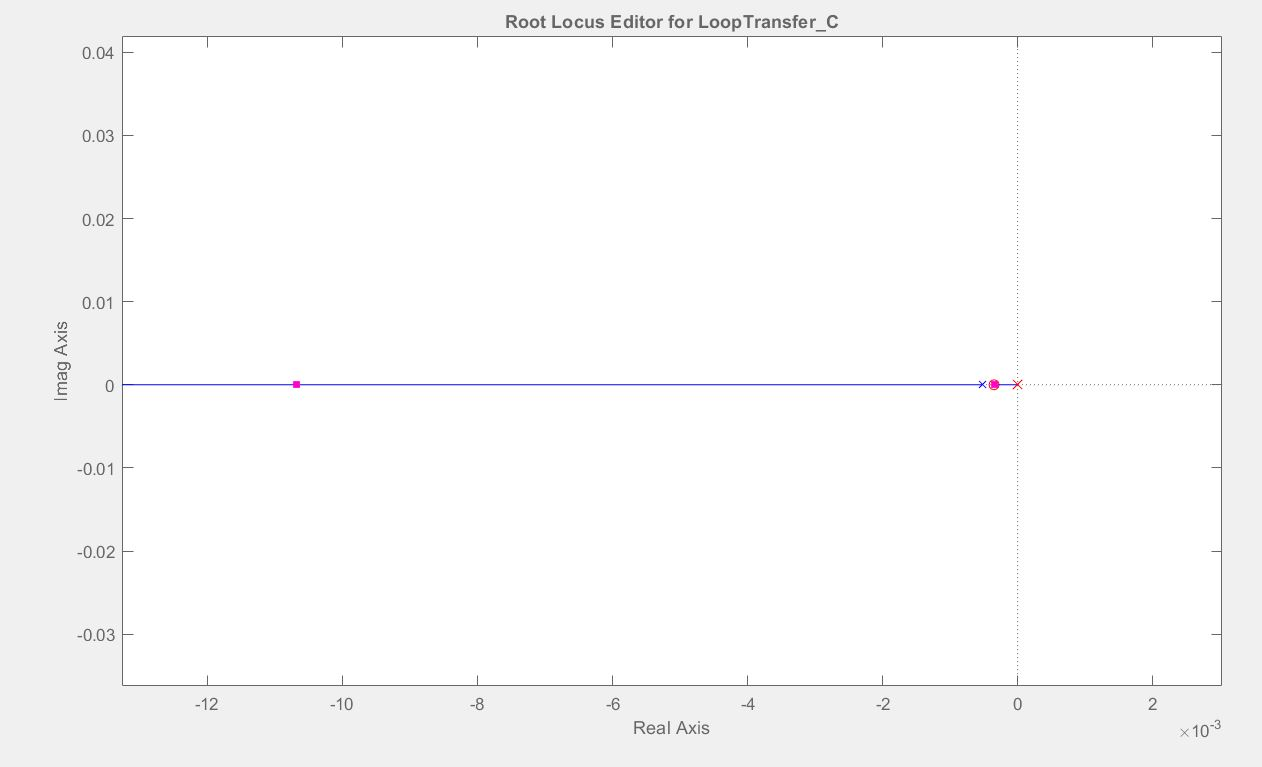
\includegraphics[width=0.85\linewidth]{./img/RootLocus.jpg}
	\end{center}
	%\legend{Fonte: Adaptado de \citeonline{Rosario2005}.}
\end{figure}

Na Figura \ref{StepResponse} é apresentada a resposta ao salto simulada onde nota-se que a acomodação do sistema acontece com aproximadamente 800 segundos sem \textit{overshoot}, ou seja, a dinâmica da planta é 5 vezes mais rápida utilizando o controlador escolhido. 

\begin{figure}[htb]
	\caption{\label{StepResponse}Resposta ao salto simulada utilizando a ferramenta \textit{rltool}.}
	\begin{center}
	    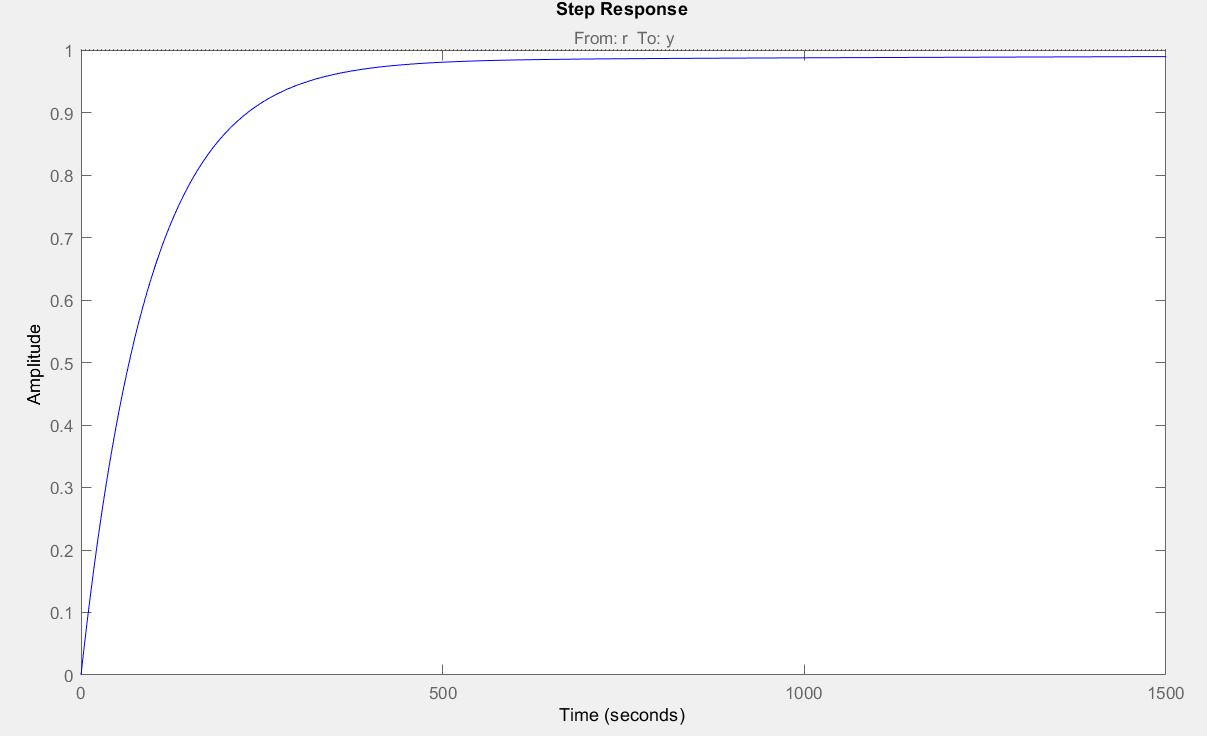
\includegraphics[width=0.85\linewidth]{./img/StepResponse.jpg}
	\end{center}
	%\legend{Fonte: Adaptado de \citeonline{Rosario2005}.}
\end{figure}

%-----------------------------------------------------------------------------------------------------------------------------------
		\section{Equação de Recorrência}
%-----------------------------------------------------------------------------------------------------------------------------------
Conforme apresentado no capítulo anterior, o controlador escolhido será implementado de forma digital na placa Arduino Uno. Desta forma, a função de transferência (\ref{eq:10}) deve ser discretizada e a saída do controlador escrita como uma equação de recorrência. A técnica utilizada foi o retentor de ordem zero, implementada em MATLAB a partir da função \textit{c2d}. Nesta função, os argumentos de entrada são o modelo contínuo, o período de amostragem e o método de conversão. Portanto, utilizando como modelo contínuo a equação (\ref{eq:10}), tempo de amostragem de 5 segundos e como método o retentor de ordem zero foi obtido o seguinte modelo discretizado:

\begin{equation}
	\label{eq:11}
	C(z)=\frac{U(z)}{E(z)} =\frac{5.25z-5.248}{z-1}.
\end{equation}

A função de transferência (\ref{eq:11}) pode ser reescrita como uma equação de recorrência simplesmente aplicando a transformada Z inversa sobre ela: 

\begin{equation}
	\label{eq:12}
	u[n]=u[n-1]+5.25 e[n]-5.248 e[n-1].
\end{equation}

Percebe-se que essa subtração possui está na 3 casa decimal, portanto é necessário ter atenção ao implementar no microcontrolador para não haver erro numérico causado pelo ponto flutuante.
%-----------------------------------------------------------------------------------------------------------------------------------
		\section{Validação experimental}
%-----------------------------------------------------------------------------------------------------------------------------------
\begin{comment}
Primeiramente foi desenvolvida uma rotina em \textit{MATLAB} para simular a ação do controlador. Para isso a função de transferência da planta foi discretizada da mesma forma que o controlador. Na equação \ref{eq:13} está a função de transferência mostrada em \ref{eq:9} em sua forma discreta.

\begin{equation}
	\label{eq:13}
	G(z)=\frac{Y(z)}{U(z)}=\frac{0.009987}{z-0.9974}
\end{equation}

Colocando a função descrita em \ref{eq:13} na forma de equação de recorrência se chega na equação \ref{eq:14}.

\begin{equation}
	\label{eq:14}
	y[n]=0.9974 y[n-1] + 0.009987 u[n-1]
\end{equation}

Percebe-se que $y[n]$ é a temperatura na interação de número $n$ e que $u[n-1]$ é o sinal de controle em uma amostragem anterior. Portanto, realizando uma rotina que efetue as interações da equação \ref{eq:14} e \ref{eq:12} é possível simular o comportamento da planta e do controlador interagindo. Essa simulação é apresentada na figura \ref{simulacaoControlador}.

Analisando a figura \ref{simulacaoControlador} se percebe que a temperatura inicial é de 55 °C. Foi realizado desta maneira para que a simulação se aproximasse de uma subida entre uma rampa de 55 °C para uma rampa de 65 °C. Outro aspecto é o tempo de acomodação que, embora seja maior que o do modelo da planta, tem valor de aproximadamente 15000 segundos para a tolerância de 1 °C. Este é um tempo elevado considerando uma mosturação com tempo máximo de 2 horas. Entretanto, o modelo considera um sistema linear, onde a abertura em graus do registro de gás varia linearmente a temperatura, na prática isto não acontece, assim sendo necessário o teste no sistema físico.


\begin{figure}[htb]
	\caption{\label{simulacaoControlador}Simulação do controlador.}
	\begin{center}
	    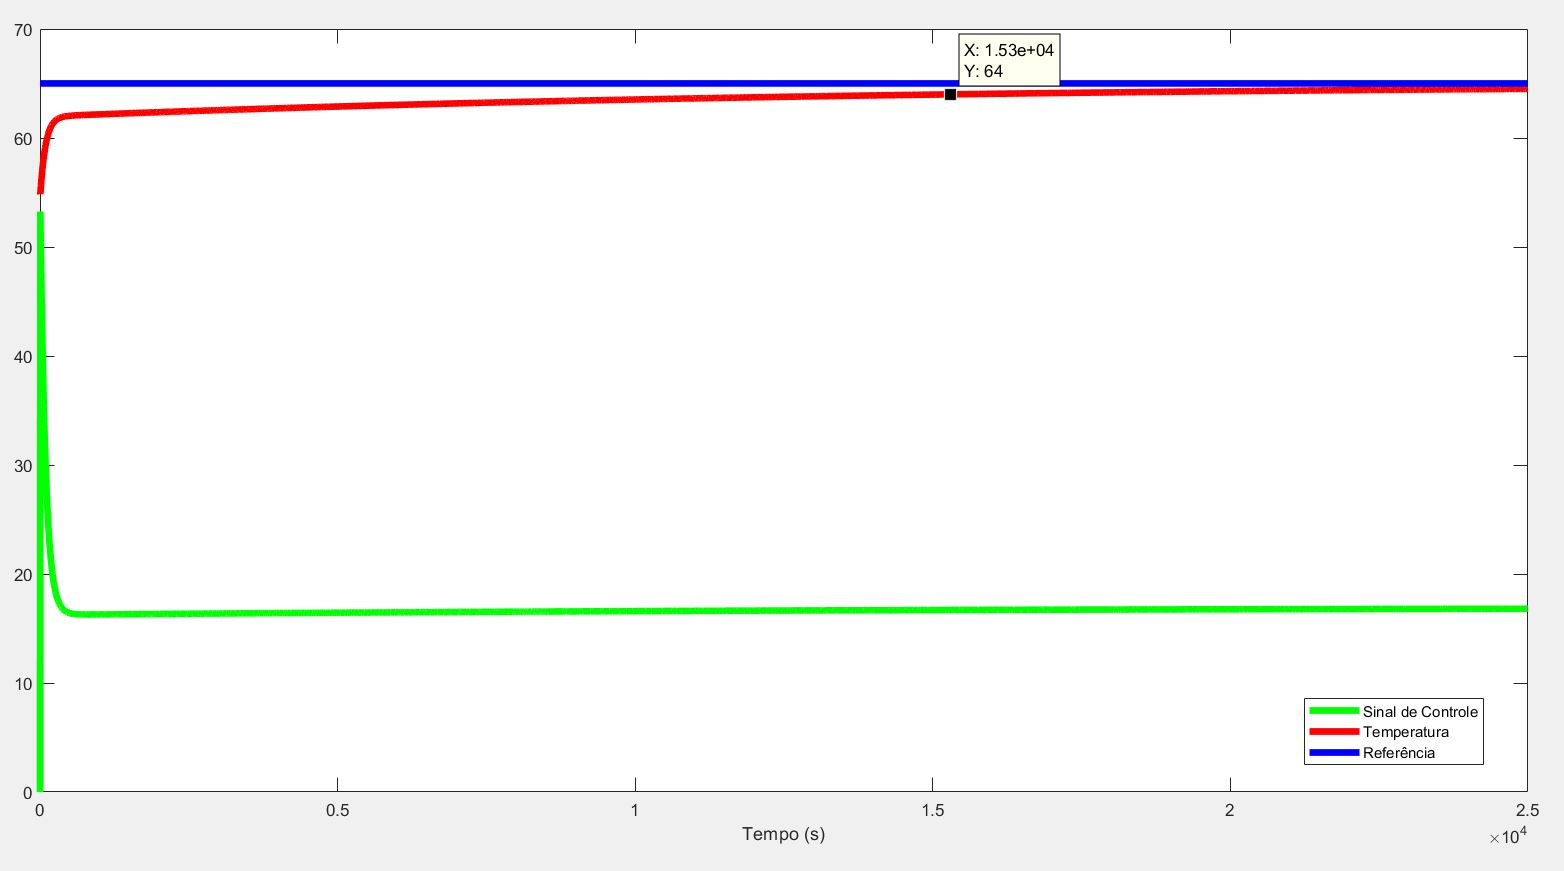
\includegraphics[width=0.9\linewidth]{./img/simulacaoControlador.jpg}
	\end{center}
	%\legend{Fonte: Adaptado de \citeonline{Rosario2005}.}
\end{figure}
\end{comment}


O teste foi realizado da mesma maneira dos testes para a determinação do modelo da planta. No módulo intermediário do \textit{brewstand} e utilizando o caldeirão de mostura com 30 litros de água e recirculação ligada. O botijão de gás estava com metada da carga total, temperatura ambiente de aproximadamente 20 graus. Elevou-se a temperatura para aproximadamente 55°C e foi ligado o controle de temperatura(implementado na placa de desenvolvimento \textit{arduino}) com referência de 65°C. É importante ressaltar que havia, durante o teste, presença de chama piloto. 

Na Figura \ref{testeControlador}, pode-se ver o teste realizado com o controlador e a planta. Nota-se que o tempo de acomodação é 25\% menor do que o obtido em simulação. Outro fator importante é a não existência de \textit{overshoot}, assim, em casos onde a rampa seja próxima da temperatura de denaturação das enzimas, não corra o risco destas perderem sua função. Esta diferença entre simulação e prática é decorrente de não linearidades entre a abertura do registro e a vazão de gás resultante. Verificou-se que, a partir de uma abertura em graus do registro (10 graus, aproximadamente), a vazão de saída do gás é muito mais elevada quando comparada a pequenos valores de curso da válvula. Na Figura \ref{curvaValvula} é a apresentada a curva de variação da vazão em relação ao curso de abertura de diferentes tipos válvulas. A válvula utilizada é do tipo bola, tendo o seu comportamento descrito pela curva em azul. Uma alternativa seria o levantamento experimental da curva de vazão da válvula utilizada e a criação de uma função para compensação do sinal de controle a partir desta função. Visando manter a estrutura de controle mais simples possível e como os resultados verificados foram satisfatórios, essa função de correção não foi implementada. Durante o teste houve um erro de comunicação durante cerca de 1 minuto e alguns dados foram perdidos, ocasionando a inclinação abrupta perto dos 600 segundos.  

\begin{figure}[htb]
	\caption{\label{testeControlador}Teste prático do controlador.}
	\begin{center}
	    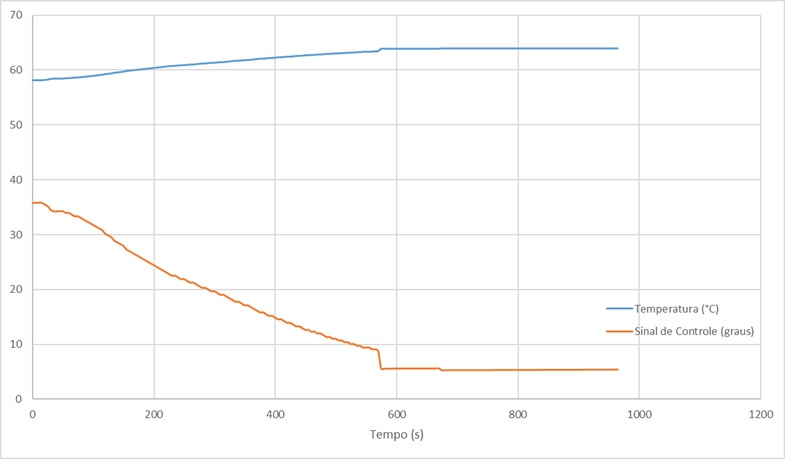
\includegraphics[width=0.9\linewidth]{./img/testeControlador.jpg}
	\end{center}
	%\legend{Fonte: Adaptado de \citeonline{Rosario2005}.}
\end{figure}

Analisando a Figura \ref{testeControlador} se verifica que o sinal de controle inicia no valor de 36 graus de abertura. Este valor está acima da saturação do registro de gás que é de, aproximadamente, 30 graus. Esta saturação é aproximada, pois foi inferida qualitativamente pela altura da chama e som de saída do gás. Embora haja a saturação do atuador, não se verifica a ocorrência de \textit{overshoot} ou dinâmicas lentas que justificariam a diminuição do ganho do controlador ou a inserção de laços de \textit{anti-windup}.



\begin{figure}[htb]
	\caption{\label{curvaValvula}Vazão pelo curso para diferentes tipos de válvula.}
	\begin{center}
	    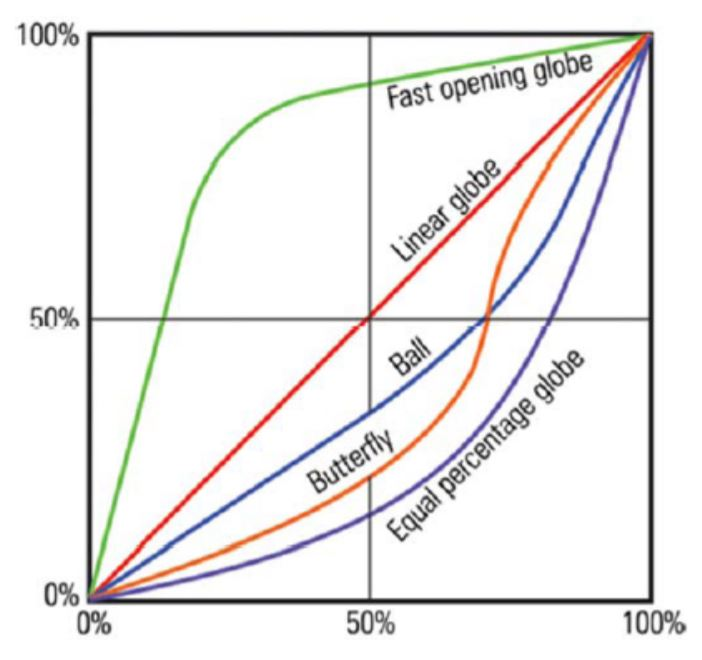
\includegraphics[width=0.55\linewidth]{./img/curvaValvulas.jpg}
	\end{center}
	\legend{Fonte: Universidade Tecnológica Federal do Paraná - Coordenação de Engenharia Eletrônica -  Aula 7 - Prof. Leandro Castilho Brolin.}
\end{figure}

%=========================================================================
	\chapter{Solução de Software}
%=========================================================================
A automação e IHM do processo de fabricação da cerveja é baseada em um supervisório. Neste capítulo serão explicadas as funcionalidades deste supervisório e a sua lógica de funcionamento.


%=========================================================================
	\section{Máquina de Estados}
%=========================================================================
Foram automatizadas as etapas de mosturação, lavagem, fervura e resfriamento do processo de fabricação de cerveja. Portanto, é possível descrever o funcionamento da automação do sistema através de uma máquina de estados com as ações que o supervisório deve tomar. Na Figura \ref{fluxograma} está um esboço do projeto funcional onde algumas ações são sequênciais, como o fechamento da primeira válvula ocasionando a abertura da segunda. Acontecem ações paralelas, como o controle de temperatura do caldeirão 1 e caldeirão 2 que ocorrem simultaneamente durante o estado "Mostura 1". Outras ações são ocasionas pelos sinais dos sensores ou devido a passagem de uma quantidade de tempo predeterminada, como no caso do fechamento fechamento do registro de gás 3 no estado "Fervura".  A seguir serão detalhados os estados e os sinais envolvidos.

\begin{figure}[htb]
	\caption{\label{fluxograma}Máquina de Estados.}
	\begin{center}
	    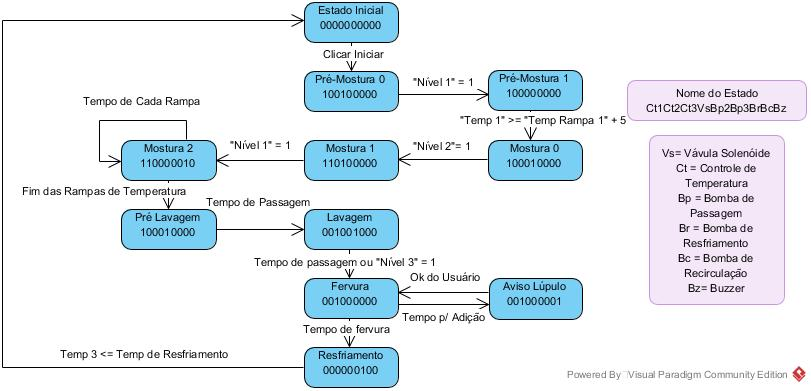
\includegraphics[width=1\linewidth]{./img/MaquinadeEstados.JPG}
	\end{center}
	%\legend{Fonte: Adaptado de \citeonline{Rosario2005}.}
\end{figure}

\begin{itemize}
	   \item \textbf{Estado Inicial:} Não possui nenhum atuador ligado. Estado onde o usuário está selecionando os valores no supervisório e estabelecendo comunicação. Os dados dos sensores, assim que a comunicação é estabelecida, são enviados e mostrados no supervisório em todos os estados, incluindo o Estado Inicial. 
\end{itemize}

\begin{itemize}
	   \item \textbf{Pré-Mostura 0:} A válvula solenóide 1 é ligada e o controle de temperatura do caldeirão 1 é acionado. Nesse estado, a caldeira 1 começa a receber água do sistema de saneamento e é ligado o controle de temperatura com a referência correspondendo ao valor da primeira rampa. 
\end{itemize}

\begin{itemize}
	   \item \textbf{Pré-Mostura 1:} Entra-se nesse estado no momento que a caldeira 1 está preenchida, ou seja, o sensor de nível 1 está em nível lógico 1. Esse estado tem como objetivo esperar que a temperatura dessa caldeira chegue ao valor da primeira rampa selecionada pelo usuário.
\end{itemize}

\begin{itemize}
	   \item \textbf{Mostura 0:} Quando a temperatura da caldeira 1 chega no valor da primeira rampa, a bomba de transferência 2 é acionada. Dessa forma a água que está aquecida na caldeira 1 é transferida para a caldeira 2, onde está o malte.
\end{itemize}

\begin{itemize}
	   \item \textbf{Mostura 1:} Assim que o nível do caldeirão 2 é atingido o estado de Mostura 1 começa e a válvula 1 é acionada. Este é um estado apenas para preencher o caldeirão 1 com água para se preparar para lavagem. 
\end{itemize}

\begin{itemize}
	   \item \textbf{Mostura 2:} Tem como objetivo implementar as rampas de temperaturas escolhidas pelo usuário. Quando cada tempo em uma temperatura passa, é mudada a referência para um novo valor predeterminado pelo usuário. Quando todas as rampas forem implementadas, ocorre a transição para o próximo estado.
\end{itemize}

\begin{itemize}
	   \item \textbf{Pré-Lavagem:} Para uma melhor lavagem dos grãos, primeiro é retirado todo o líquido do caldeirão 2 e passado para o caldeirão 3. Este estado mantém ligada a bomba de transferência 3 durante um tempo de 3 minutos, estabelecido empiricamente como o tempo necessário para completar a transferência.
\end{itemize}

\begin{itemize}
	   \item \textbf{Lavagem:} Na lavagem, água a 78°C é passada sobre o malte com objetivo de retirar o açúcar residual dos grãos. Neste estado as bombas de transferência 2 e 3 estão ligadas, de forma que a água que está a 78°C no caldeirão 1 é transferida para o caldeirão 2. A água é largada sobre os grãos e retirada no inferior do caldeirão 2, sendo transferida para o cadeirão 3. O fim da lavagem é determinado por tempo, arbitrado em 5 minutos. 
\end{itemize}

\begin{itemize}
	   \item \textbf{Fervura:} Na fervura, o único atuador que é acionado é o servomotor. O servomotor responsável pela abertura do registro de gás para ferver o mosto presente no caldeirão 3. Este estado finaliza quando o tempo determinado pelo usuário esgotar. 
\end{itemize}

\begin{itemize}
	   \item \textbf{Aviso Lúpulo:} Dependo da receita da cerveja, o lúpulo deve ser adicionado em momentos específicos definidos pelo usuário. Quando um lúpulo deve ser adicionado este estado é acionado. Ele mantém um \textit{buzzer} ativo enquanto o usuário não clicar em "OK" no aviso da figura \ref{mensagemlupulo}.
\end{itemize}

\begin{itemize}
	   \item \textbf{Resfriamento:} O último estado é o de Resfriamento. Nele a bomba de resfriamento é ligada, a qual bombeia água fria em uma serpentina posicionada dentro do caldeirão 3, desta forma resfriando o mosto. Ele acaba quando a temperatura do caldeirão 3 é menor que a selecionada pelo usuário. Assim que acaba é retornado para o estado inicial fechando o ciclo da máquina de estados.  
\end{itemize}




%=========================================================================
		\section{Descrição do supervisório}
%-----------------------------------------------------------------------------------------------------------------------------------

Utilizando o Visual Studio 2010 foi construído um programa supervisório que, além de mostrar os dados da planta, implementa a lógica da máquina de estados da Figura  \ref{fluxograma}. A interface do programa é apresentada na Figura \ref{Supervisorio}. Nela é possível adicionar as temperaturas desejadas nas rampas, além da temperatura de resfriamento, tempo de fervura e os tempos em que serão adicionados os lúpulos. Nesta tela são mostradas as temperaturas de cada caldeirão e os estados dos sensores de chama e nível.

\begin{figure}[htb]
	\caption{\label{Supervisorio}Tela do programa supervisório.}
	\begin{center}
	    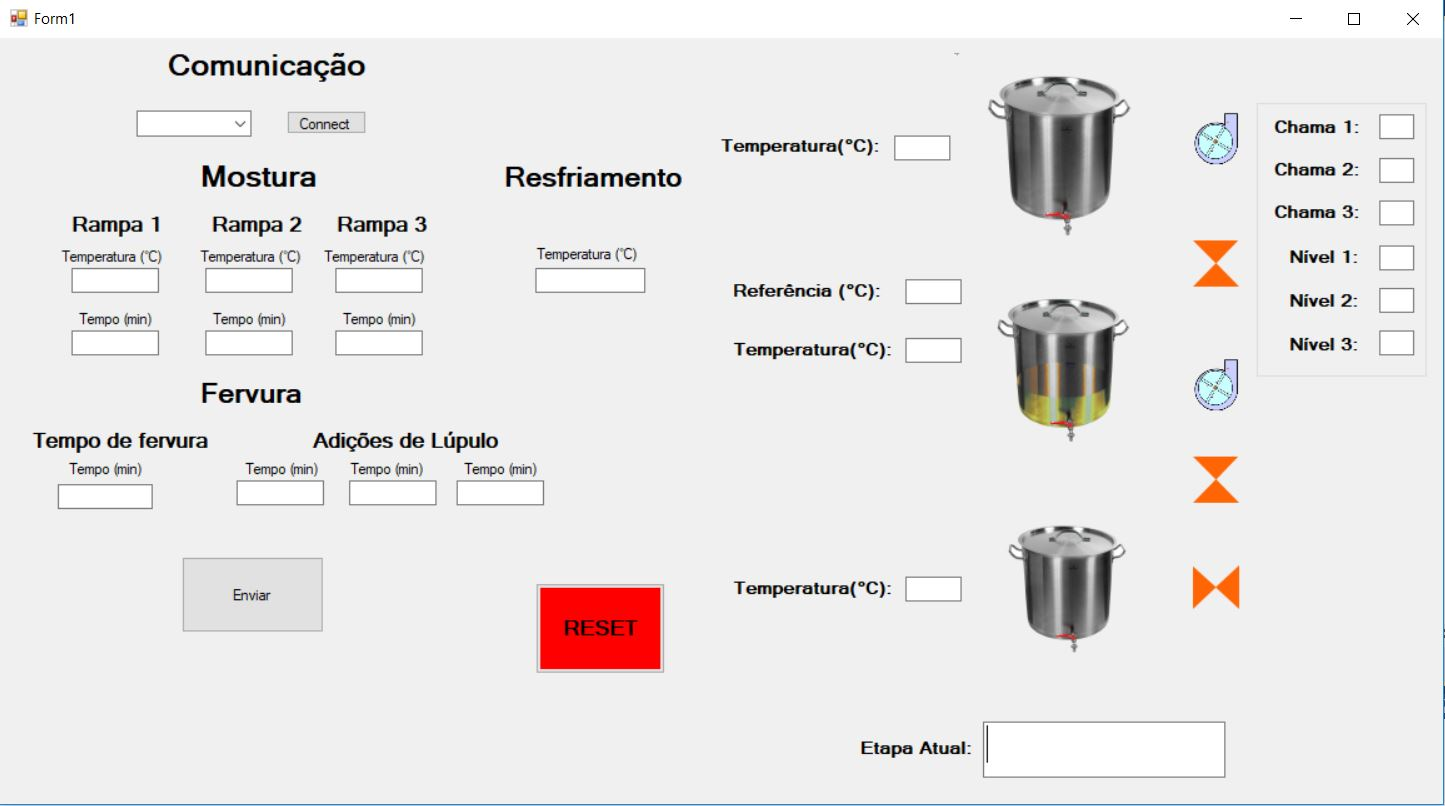
\includegraphics[width=0.95\linewidth]{./img/Supervisorio.jpg}
	\end{center}
	%\legend{Fonte: Adaptado de \citeonline{Rosario2005}.}
\end{figure}

Quando estão cheios, os caldeirões são mostrados em coloração azul, ilutrado na Figura \ref{Supervisorio02}. Caso a válvula solenóide ou as bombas de passagem estiverem ligadas, elas aparecem em verde e se fechadas, em vermelho. Caso a bomba de resfriamento ou a bomba de recirculação estiverem ligadas elas aparecem se movimentando. Finalmente, se o caldeirão estiver com controle de temperatura acionado, uma chama irá aparecer sob ele.

\begin{figure}[htb]
	\caption{\label{Supervisorio02}Representação gráfica dos caldeirões cheios e das chamas acesas.}
	\begin{center}
	    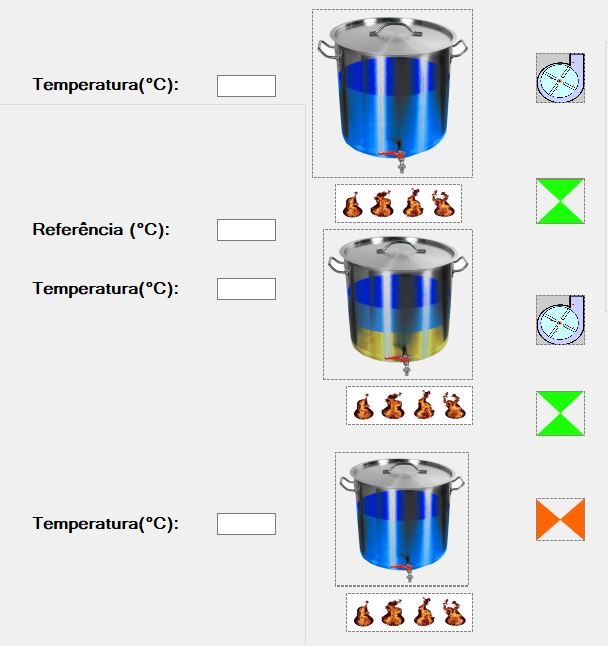
\includegraphics[width=0.7\linewidth]{./img/Supervisorio02.jpg}
	\end{center}
	%\legend{Fonte: Adaptado de \citeonline{Rosario2005}.}
\end{figure}

%=========================================================================
		\section{Funcionalidades}
%-----------------------------------------------------------------------------------------------------------------------------------
\begin{itemize}
\item \textbf{Comandos:}
O programa supervisório é responsável pelo gerenciamento dos acionamentos dos atuadores. Ele recebe os dados dos sensores via comunicação serial com o \textit{Arduino} e a partir desses dados decide os comandos que serão enviados para o microcontrolador executar. Não é possível para o usuário decidir qual atuador vai ser acionado em um determinado instante, todas as decisões são implementadas seguindo a máquina de estados da Figura \ref{fluxograma}. 
\end{itemize}

\begin{itemize}
\item \textbf{Comunicação:}
A comunicação é via serial com \textit{baudrate} de 9600 $bits/s$. Os dados são enviados em uma palavra de tamanho fixo a cada segundo. A palavra inicia com a letra "a" e finaliza com a letra "b", sendo "a" sempre o primeiro caracter e "b" o décimo quinto. Entre esses caracteres são enviados números 0 ou 1 para o acionamento dos atuadores e também é enviado dois caracteres com a informação da referência de temperatura do controle do caldeirão 1 e caldeirão 2. Essa técnica poderia ser substituida ou melhorada utilizando \textit{checksum}, ou seja, somando os valores dos dados que serão enviados e enviar este somatório junto, o receptor, ao receber os dados, faz o mesmo somatório e checa com o valor da soma que foi enviado.

O microcontrolador, ao receber essa palavra, verifica o primeiro e último caracter. Estando corretos, ele verifica se a combinação de acionamentos está entre as combinações possíveis, e previamente registradas em sua memória. Isto é realizado para garantir que nenhum atuador será ligado no momento errado. Antes de implementar esta rotina, em certos momentos, valores aleatórios eram enviados, ocasionando o acionamento incorreto das válvulas e bombas. Pode-se ver na Figura \ref{palavra} a palavra enviada, sendo SM abreviação para servomotor, VS para válvula solenóide, Ref. para referência de temperatura do caldeirão, Rec. para recirculação e Resf. para resfriamento.

\begin{figure}[htb]
	\caption{\label{palavra}Palavra enviada via serial.}
	\begin{center}
	    \includegraphics[width=1\linewidth]{./img/palavra.jpg}
	\end{center}
	%\legend{Fonte: Universidade Tecnológica Federal do Paraná - Coordenação de Engenharia Eletrônica -  Aula 7 - Prof. Leandro Castilho Brolin.}
\end{figure}

\end{itemize}

\begin{itemize}
\item \textbf{Registro dos dados:}
Os dados de temperatura dos sensores são gravados a cada 10 segundos em um arquivo texto. Verifica-se que este tempo de registro é diferente do período de amostragem do controlador que é de 5 segundos. Neste mesmo arquivo é registrada a data e horário de início e de fim. O início do processo é considerado ao clicar no botão "Enviar" e o fim ao receber a mensagem da Figura \ref{mensagemdefim}. 

  \begin{figure}[htb]
	\caption{\label{mensagemdefim}Mensagem de fim do processo.}
	\begin{center}
	    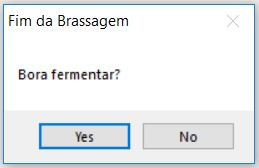
\includegraphics[width=0.25\linewidth]{./img/mensagemdefim.jpg}
	\end{center}
	%\legend{Fonte: Universidade Tecnológica Federal do Paraná - Coordenação de Engenharia Eletrônica -  Aula 7 - Prof. Leandro Castilho Brolin.}
\end{figure}
\end{itemize}

%=========================================================================
		\section{Tela e Operação}
%-----------------------------------------------------------------------------------------------------------------------------------
Baseado na Figura \ref{Supervisorio}, verifica-se no canto esquerdo superior uma caixa de seleção e, ao lado, um botão. Nesta caixa aparecem as portas seriais disponiveis para conexão. O usuário deve escolher a porta onde está conectado o microcontrolador e clicar no botão. Quando isto acontece, inicia a troca de dados entre supervisório e microcontrolador, aparecem as temperaturas ao lado de cada caldeirão e o estado dos sensores de nível e chama. Este é o primeiro passo que o usuário deve realizar.

Após estabelecer a conexão, o usuário deve fornecer os dados das rampas (temperatura e tempo), a temperatura de resfriamento, tempo de fervura e os tempos das adições de lúpulo. Ao menos uma rampa e uma adição de lúpulo devem ser selecionados, caso isto não aconteça, não é possível realizar o envio dos dados. Se o usuário não adicionar a temperatura de resfriamento ou o tempo de fervura são considerados a temperatura de 20 °C e o tempo de 60 minutos de fervura. Quando o botão enviar é pressionado e todos os dados necessários estão preenchidos, a mensagem da Figura \ref{mensagemdeinicio} aparece e o processo inicia. 

  \begin{figure}[htb]
	\caption{\label{mensagemdeinicio}Mensagem de início do processo.}
	\begin{center}
	    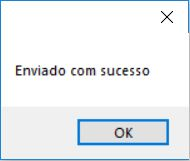
\includegraphics[width=0.25\linewidth]{./img/mensagemdeinicio.jpg}
	\end{center}
	%\legend{Fonte: Universidade Tecnológica Federal do Paraná - Coordenação de Engenharia Eletrônica -  Aula 7 - Prof. Leandro Castilho Brolin.}
\end{figure}

O botão de \textit{Reset}, que está em vermelho, pode ser pressionado a qualquer momento. Caso ele seja pressionado, todos os atuadores são desligados e o sistema volta ao estado inicial, não sendo possível retomar do estado em que se encontrava.

Após iniciar o processo o usuário só volta a interagir com o supervisório nas adições de lúpulo. No momento que uma adição deve ocorrer, o aviso da Figura \ref{mensagemlupulo} aparece. Enquanto não é pressionado o botão "OK", o \textit{buzzer} fica acionado. Quando o botão é pressionado o aviso desaparece e o \textit{buzzer} é desligado.

  \begin{figure}[htb]
	\caption{\label{mensagemlupulo}Mensagem para adição de lúpulo.}
	\begin{center}
	    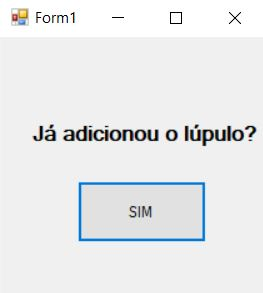
\includegraphics[width=0.25\linewidth]{./img/mensagemlupulo.jpg}
	\end{center}
	%\legend{Fonte: Universidade Tecnológica Federal do Paraná - Coordenação de Engenharia Eletrônica -  Aula 7 - Prof. Leandro Castilho Brolin.}
\end{figure}
%=========================================================================
	\chapter{Teste de operação}
%=========================================================================
De uma forma geral, os parâmetros utilizados na avaliação da repetibilidade do processo de brassagem são a medida de eficiência do processo como um todo e pelos perfis de temperatura de cada caldeirão. Outra avaliação, porém qualitativa, é pelo sabor, corpo e espuma da cerveja. A eficiência é calculada utilizando a massa do malte, densidade do mosto após a fervura e o volume após a fervura, representando assim o quanto de açúcar, proteína e outros compostos solúveis foram passados do malte para o mosto. Vale ressaltar que no processo de maltagem moderna, os maltes são mais homogêneos e a temperatura da mosturação não interfere tanto na eficiência. Pode-se avaliar a repetibilidade do processo pela temperatura, utilizando sempre as mesmas rampas programadas, a mesma quantidade de malte e tempo de fervura. As temperaturas de duas brassagens devem ser iguais ou muito próximas para ter uma repetibilidade aceitável. 

Devido aos custos e demora do processo de brassagem, apenas três testes serão apresentados.

%=========================================================================
	\section{Teste 1}
%=========================================================================
Para o primeiro teste o equipamento foi limpo e configurado conforme descrito no Capítulo 3. Foram inseridos 2 litros de água em cada caldeirão e uma chama piloto foi acesa sob cada um deles. Dessa forma, quando o registro de gás é aberto inicia-se a combustão, evitando a necessidade de ignição manual para o teste. Os 2 litros de água impedem o superaquecimento do sistema que poderia ser causado pela chama piloto. Foram inseridos 6kg de malte na caldeira 2 e a serpentina de resfriamento na caldeira 3. Configurou-se os parâmetros da Tabela \ref{Configuracoes} no supervisório e se iniciou o processo. 

  \begin{figure}[htb]
	\caption{\label{teste01c1}Temperatura do caldeirão 1 no teste 1.}
	\begin{center}
	    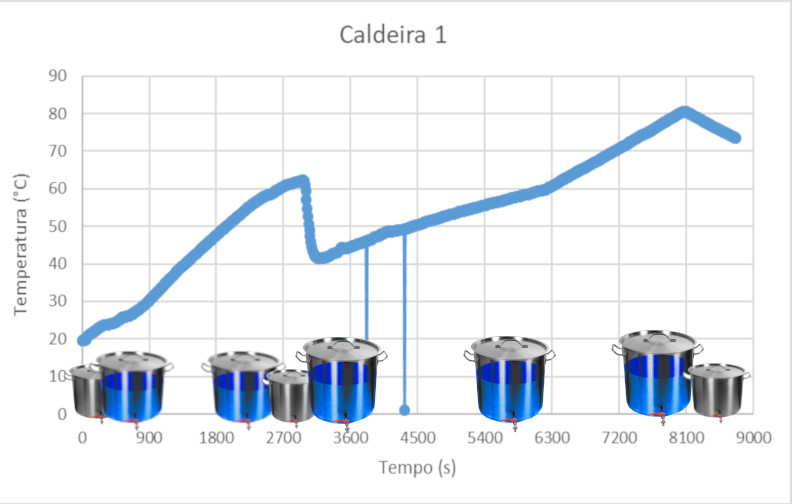
\includegraphics[width=0.95\linewidth]{./img/teste01_cald1.jpg}
	\end{center}
	%\legend{Fonte: Universidade Tecnológica Federal do Paraná - Coordenação de Engenharia Eletrônica -  Aula 7 - Prof. Leandro Castilho Brolin.}
\end{figure}

  \begin{figure}[htb]
	\caption{\label{teste01c2}Temperatura do caldeirão 2 no teste 1.}
	\begin{center}
	    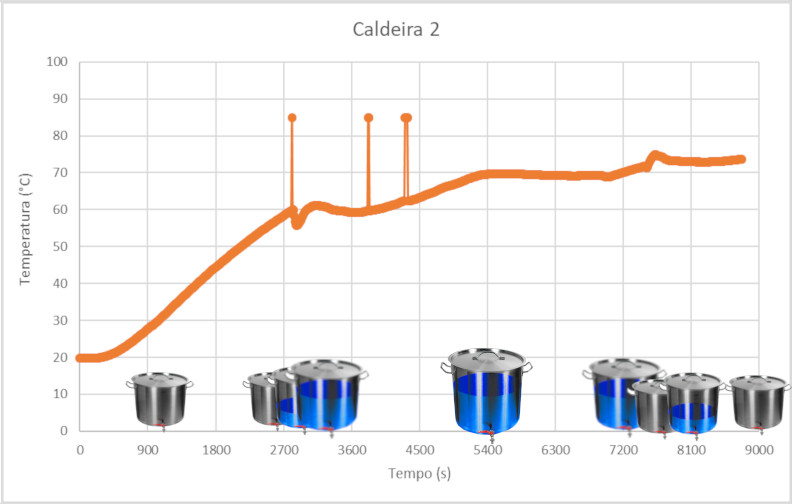
\includegraphics[width=0.95\linewidth]{./img/teste01_cald2.jpg}
	\end{center}
	%\legend{Fonte: Universidade Tecnológica Federal do Paraná - Coordenação de Engenharia Eletrônica -  Aula 7 - Prof. Leandro Castilho Brolin.}
\end{figure}

\begin{table}[]
\centering
\caption{Configurações dos Teste 1, 2 e 3.}
\label{Configuracoes}
\begin{tabular}{cc}
\hline
\textbf{Configuração}    & \textbf{Valor} \\ \hline
Temperatura Rampa 1      & 55 °C          \\ \hline
Temperatura Rampa 2      & 65 °C          \\ \hline
Temperatura Rampa 3      & -              \\ \hline
Tempo Rampa 1            & 15 min         \\ \hline
Tempo Rampa 2            & 45 min         \\ \hline
Tempo Rampa 3            & -              \\ \hline
Temperatura de Resf.     & 25 °C          \\ \hline
Tempo de Fervura         & 60 min         \\ \hline
Tempo Adição de Lúpulo 1 & 60 min         \\ \hline
Tempo Adição de Lúpulo 2 & 45 min         \\ \hline
Tempo Adição de Lúpulo 3 & 30 min         \\ \hline
\end{tabular}
\end{table}

Neste teste não havia controle proporcional-integral implementado no Arduino. Portanto o controle de temperatura foi realizado através de controlador bang-bang, ou seja, enquanto a temperatura estava abaixo da referência o registro era aberto a 25° e, quando a temperatura estava acima, este era fechado. É importante ressaltar que o botijão de gás utilizado estava com carga baixa durante o teste.

Utilizou-se a temperatura da primeira rampa + 5°C neste teste, pois era esperado uma diminuição de temperatura devido a transferência, assim quando a água da caldeira 1 preenchesse a caldeira 2 haveria troca de calor entre o líquido e o malte e estes estabilizariam na temperatura da primeira rampa. Mas neste teste se percebeu que não há alteração durante a troca de líquidos entre as caldeiras, portanto foi retirada essa adição de 5°C nos próximos testes. 

Na Figura \ref{teste01c1} está o perfil de temperatura do caldeirão 1, abaixo da curva estão os estados do caldeirão. Inicialmente a caldeira está vazia, é preenchida de água e aquecida até a temperatura equivalente a primeira rampa de temperatura + 5 °C. Quando a temperatura é atingida (2700 segundos) ocorre a transferência de líquido da caldeira 1 para 2. Finalizada a transferência a caldeira 1 é preenchida com água do sistema de saneamento e tem sua temperatura abruptamente diminuída (2800 segundos). Quando o nível do caldeirão está completo o registro de gás é aberto e inicia o controle de temperatura com referência de 78°C (Temperatura para lavagem dos grãos). Alcançanda a temperatura é iniciada a etapa de lavagem, onde ocorre a transferência da caldeira 1 para 2, assim abaixando a temperatura novamente.


Na Figura \ref{teste01c2} está o perfil de temperatura do caldeirão 2, abaixo da curva estão os estados do caldeirão. Inicialmente a caldeira está vazia, esta recebe água aquecida da caldeira 1 (2770 segundos), quando a água é inserida na caldeira 2, ela atravessa o malte que está em baixa temperatura, causando a depressão de temperatura vista no gráfico aos 2800 segundos. Conforme o volume de água aumenta essa temperatura se estabiliza. A primeira rampa começa em 2860 segundos e é finalizada em 3760 segundos. Quando finalizada é iniciado o aquecimento para se alcançar o patamar da segunda rampa (65°C). Devido a inércia térmica percebe-se que acontece um \textit{overshoot} alcançando os 70°C. Aos 7200 segundos o mosto da caldeira 2 é transferido para 3 e aos 7500 segundos o processo de lavagem é iniciado, causando a elevação da temperatura.

Finalizando a lavagem a fervura é iniciada, são contados 60 minutos assim que a temperatura do caldeirão 3 atinge 98°C. O teste iniciou 8h50min e acabou 12h52min, durando 4 horas descontando o tempo da etapa de resfriamento que não foi realizada. 


%=========================================================================
	\section{Teste 2}
%=========================================================================

No segundo teste o equipamento foi limpo e configurado conforme o Capítulo 3. Foram inseridos 2 litros de água em cada caldeirão e uma chama piloto foi acesa sob cada um deles. Neste teste não havia malte na caldeira 2 e a serpentina de resfriamento foi inserida na caldeira 3 desde o início da fabricação. Configurou-se os parâmetros no supervisório e se iniciou o processo. 
  \begin{figure}[htb]
	\caption{\label{teste02c1}Temperatura do caldeirão 1 no teste 2.}
	\begin{center}
	    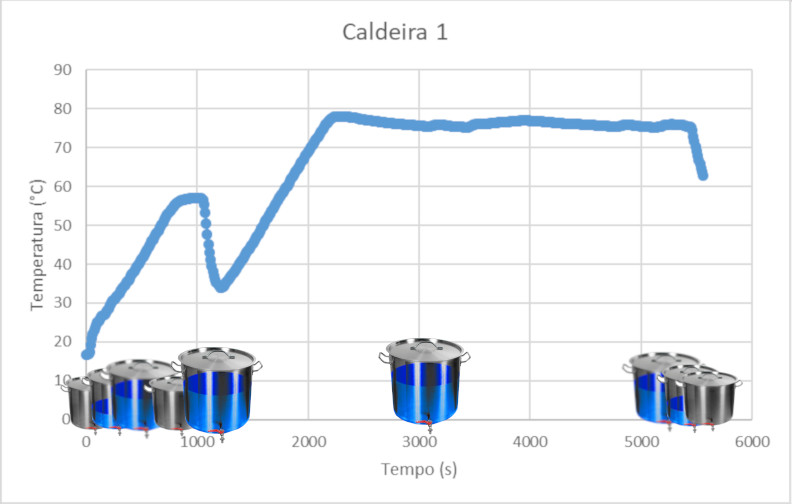
\includegraphics[width=0.95\linewidth]{./img/teste02_cald1.jpg}
	\end{center}
	%\legend{Fonte: Universidade Tecnológica Federal do Paraná - Coordenação de Engenharia Eletrônica -  Aula 7 - Prof. Leandro Castilho Brolin.}
\end{figure}
O controle proporcional-integral estava implementado no Arduino e foi utilizado o mesmo controlador para o caldeirão 1 e 2, sendo inseridos saltos na referência para a troca de rampas e no controle de temperatura da primeira caldeira. É importante ressaltar que o botijão de gás utilizado estava com carga total e, por esta razão, houve um aquecimento mais acelerado em relação ao Teste 1.

Na Figura \ref{teste02c1} está o perfil de temperatura do caldeirão 1, abaixo da curva estão os estados do caldeirão. Inicialmente a caldeira está vazia, é preenchida de água e, em seguida, aquecida até a temperatura equivalente a primeira rampa de temperatura. Percebe-se que há \textit{overshoot} em relação a configuração escolhida para rampa 1. Quando a temperatura é ultrapassada (950 segundos) ocorre a transferência de líquido da caldeira 1 para 2. Finalizada a transferência a caldeira 1 é preenchida com água do sistema de saneamento (1050 segundos) e, por esta razão, tem sua temperatura abruptamente diminuída. Quando o seu nível está completo, o registro de gás é aberto e inicia o controle de temperatura com referência de 78°C (Temperatura para lavagem dos grãos). Alcançando a temperatura é esperada a etapa de lavagem, onde ocorre a transferência da caldeira 1 para 2, assim abaixando a temperatura novamente (5400 segundos).


  \begin{figure}[htb]
	\caption{\label{teste02c2}Temperatura do caldeirão 2 no teste 2.}
	\begin{center}
	    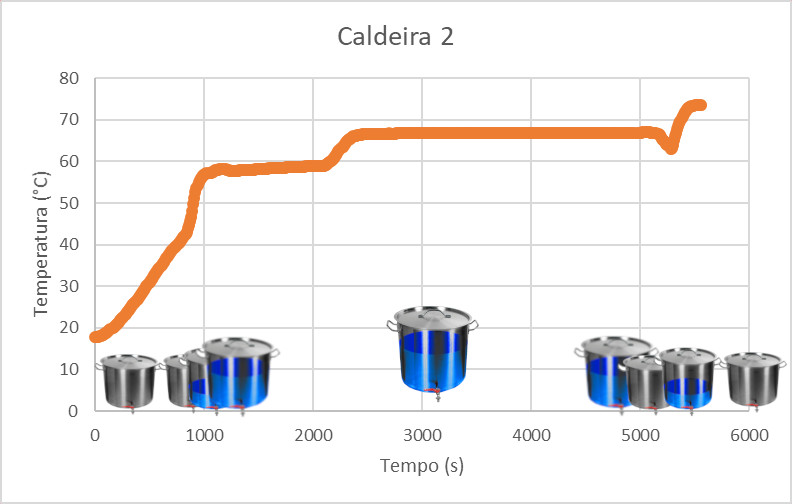
\includegraphics[width=0.95\linewidth]{./img/teste02.jpg}
	\end{center}
	%\legend{Fonte: Universidade Tecnológica Federal do Paraná - Coordenação de Engenharia Eletrônica -  Aula 7 - Prof. Leandro Castilho Brolin.}
\end{figure}


Na Figura \ref{teste02c2} está o perfil de temperatura do caldeirão 2, abaixo da curva estão os estados do caldeirão. Inicialmente a caldeira está vazia, esta recebe água aquecida da caldeira 1 (900 segundos), quando a água é inserida na caldeira 2, ela está em maior temperatura causando a mudança na inclinação da curva. A primeira rampa começa em 1200 segundos e é finalizada em 2100 segundos. Quando finalizada é iniciado o aquecimento para se alcançar o patamar da segunda rampa (65°C). Devido a inércia térmica percebe-se que acontece um \textit{overshoot} alcançando os 67°C. Aos 5150 segundos o mosto da caldeira 2 é transferido para 3, causando uma perda de temperatura e aos 5330 segundos o processo de lavagem é iniciado, causando a elevação da temperatura.

Percebe-se que durante as rampas a temperatura continua sendo elevada mesmo estando acima da referência. A causa desta anomalia é a chama piloto estar muito elevada, não permetindo o resfriamento do sistema e mudando a dinâmica da planta.


Finalizando a lavagem a fervura é iniciada, são contados 60 minutos assim que a temperatura do caldeirão 3 atinge 98°C. O teste iniciou 18h10min e acabou 21h17min, durando 3h07min descontando o tempo da etapa de resfriamento que não foi realizada. 

%=========================================================================
	\section{Teste 3}
%=========================================================================
No terceiro teste o equipamento foi limpo e colocado na configuração já descrita no Capítulo 3. Foram colocados 2 litros de água em cada caldeirão e uma chama piloto foi acesa sob cada um deles. Foram colocados malte 7kg de malte na caldeira 2 e a serpentina de resfriamento. Configurou-se os parâmetros no supervisório e se iniciou o processo. 

O controle proporcional-integral estava implementado no Arduino e foi utilizado o mesmo controlador implementado no Teste 2. É importante ressaltar que o botijão de gás utilizado estava com carga total, para tentar simular a carga média do botijão retringida a passagem de gás no registro geral. Devido essa restrição o aquecimento deste teste foi mais lento em relação ao Teste 2.

Analisando a Figura \ref{teste03c1} vê-se que inicialmente a caldeira está vazia e é preenchida de água aos 10 segundos. O líquido é aquecido até a temperatura equivalente a primeira rampa de temperatura. Percebe-se que há \textit{overshoot} em relação a configuração escolhida para rampa 1. Quando a temperatura é ultrapassada (1150 segundos) ocorre a transferência de líquido da caldeira 1 para 2. Finalizada a transferência a caldeira 1 é preenchida com água do sistema de saneamento (1250 segundos) e, por esta razão, tem sua temperatura abruptamente diminuída. Quando o seu nível está completo, o registro de gás é aberto e inicia o controle de temperatura com referência de 78°C (Temperatura para lavagem dos grãos). Alcançando a temperatura é esperada a etapa de lavagem, onde ocorre a transferência da caldeira 1 para 2, assim abaixando a temperatura novamente (6000 segundos).
 
  \begin{figure}[htb]
	\caption{\label{teste03c1}Temperatura do caldeirão 1 no teste 3.}
	\begin{center}
	    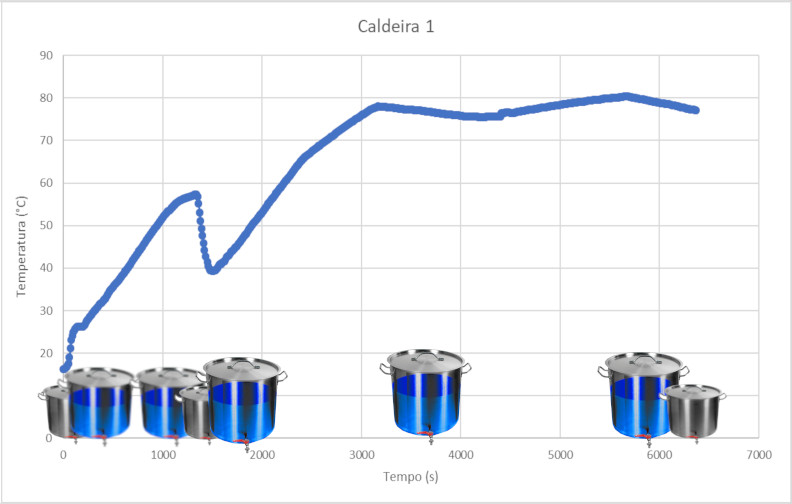
\includegraphics[width=0.95\linewidth]{./img/teste03_cald1.jpg}
	\end{center}
	%\legend{Fonte: Universidade Tecnológica Federal do Paraná - Coordenação de Engenharia Eletrônica -  Aula 7 - Prof. Leandro Castilho Brolin.}
\end{figure}

Na Figura \ref{teste03c2} está o perfil de temperatura do caldeirão 2, abaixo da curva estão os estados do caldeirão. Inicialmente a caldeira está vazia, esta recebe água aquecida da caldeira 1 aos 1150 segundos. O caldeirão 2 está com líquido em maior temperatura devido a chama piloto, quando a água da caldeira 1 é transferida eleva o nível do líquido que entra em contato com o sensor e causa um pico na curva aos 1200 segundos. Assim que toda a água é transferida e agitada a temperatura alcança os 55°C esperados. A primeira rampa começa aos 1300 segundos e é finalizada em 2200 segundos. Quando finalizada é iniciado o aquecimento para se alcançar o patamar da segunda rampa (65°C). Vê-se que após alcançar a temperatura, devido a chama piloto, a temperatura contínua sendo elevada até se estabilizar em 72°C. Aos 5900 segundos o mosto da caldeira 2 é transferido para 3, causando uma perda de temperatura e aos 6080 segundos o processo de lavagem é iniciado, causando a elevação da temperatura.

  \begin{figure}[htb]
	\caption{\label{teste03c2}Temperatura do caldeirão 2 no teste 3.}
	\begin{center}
	    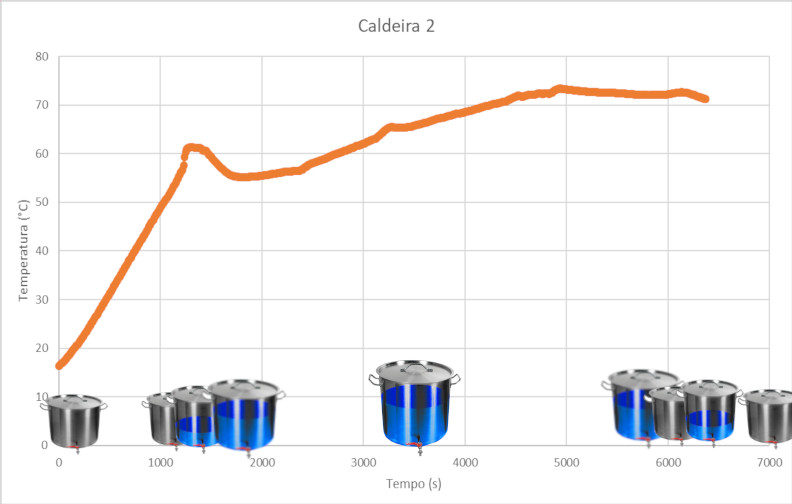
\includegraphics[width=0.95\linewidth]{./img/teste03_cald2.jpg}
	\end{center}
	%\legend{Fonte: Universidade Tecnológica Federal do Paraná - Coordenação de Engenharia Eletrônica -  Aula 7 - Prof. Leandro Castilho Brolin.}
\end{figure}

Finalizando a lavagem a fervura é iniciada, são contados 60 minutos assim que a temperatura do caldeirão 3 atinge 98°C. O teste iniciou 12h52min e acabou 17h38min, durando 4h46min contando o tempo de resfriamento. 


%=========================================================================
	\chapter{Conclusões}
%=========================================================================
O objetivo principal do trabalho é aumentar a repetibilidade, o registro dos dados e diminuir a interferência humana no processo de fabricação de cerveja caseira. Foram realizados 3 testes em uma planta caseira de 30 litros que demonstraram que o trabalho humano foi diminuído, tendo em vista que este apenas continua necessário na mistura do mosto, adição de lúpulo e limpeza do equipamento.  A partir da análise dos dados de temperatura coletados nos testes,  percebe-se que é possível ter a repetibilidade aumentada se for garantida a isonomia no fornecimento de gás. Além disso, a chama piloto considerada apresentou influência significativa no processo. O supervisório construído para a aplicação se mostrou funcional, assim como o \textit{firmware} do \textit{Arduino} e a eletrônica de acionamento. O controlador PI projetado obteve resposta satisfatória para a vazão de gás na qual a planta foi modelada, requerendo uma nova sintonia para a condição de botijão de gás cheio.

Como possíveis trabalhos futuros pode-se inserir a opção do usuário determinar o estado em que o botijão de gás se encontra, dessa forma determinando o controlador correto para a dinâmica de cada estado. Se mostrou necessária a implementação de um acendimento automático do fogo para extinguir a utilização de chama piloto, pois esta interfere na temperatura dos caldeirões. Na passagem de dados são utilizados cabos USB, sujeitando o computador a riscos devido à proximidade física do sistema. Uma forma de melhoria é a utilização de módulos Wi-Fi, permitindo o controle e monitoramento do sistema de forma remota. Também é interessante o desenvolvimento de código \textit{mobile} para controle e monitoramento via \textit{smartphones}. Afim de aumentar a eficiência do processo e diminuir ainda mais o trabalho humano, se torna interessante a instalação de equipamentos de agitação do mosto para mistura de água e grãos na mostura. 

 

%=========================================================================
% REFERÊNCIAS BIBLIOGRÁFICAS
	\postextual
	\bibliography{referencias}
%=========================================================================

\begin{comment}

%=========================================================================
% APÊNDICES
	\begin{apendicesenv}
	\partapendices
%=========================================================================
\chapter{Função em MATLAB para MTD1}
\lstinputlisting{../../MATLAB/seg_mtd1.m}
\label{ap:seg_mtd1}
%-------------------------------------------------------------------------
\chapter{Função em MATLAB para MTD2}
\lstinputlisting{../../MATLAB/seg_mtd2.m}
\label{ap:seg_mtd2}
%-------------------------------------------------------------------------
\chapter{Função em MATLAB para MTD3}
\lstinputlisting{../../MATLAB/seg_mtd3.m}
\label{ap:seg_mtd3}
%-------------------------------------------------------------------------
\chapter{Função em MATLAB para MTD4}
\lstinputlisting{../../MATLAB/seg_mtd4.m}
\label{ap:seg_mtd4}
%-------------------------------------------------------------------------
\chapter{Código em MATLAB para segmentação de sinais, treino de RNA e resultados de classificação}
\lstinputlisting{../../MATLAB/complete_mtd1.m}
\label{ap:complete_mtd1}
%-------------------------------------------------------------------------
\chapter{Código utilizado para determinação de $r_{target}$ do MTD1}
\label{ap:r_target}
\lstinputlisting{../../MATLAB/rtarget_mtd1.m}
%-------------------------------------------------------------------------
\chapter{Código utilizado para escolha de valores de $A$ do MTD2}
\label{ap:Avalue}
\lstinputlisting{../../MATLAB/A_value_mtd2.m}
%-------------------------------------------------------------------------
\chapter{Função em MATLAB para obtenção de resposta esperada de treino de RNA}
\label{ap:idMoves}
\lstinputlisting{../../MATLAB/identifyClasses.m}
%-------------------------------------------------------------------------
\end{apendicesenv}

%=========================================================================
% ANEXOS
	\begin{anexosenv}
	\partanexos
%=========================================================================
\chapter{Função em MATLAB para agrupamento com DBSCAN \cite{Thanh2013}}
\label{ap:dbscan}
\lstinputlisting{../../MATLAB/dbscan.m}
%-------------------------------------------------------------------------
\end{anexosenv}
\end{comment}


\end{document}
